\documentclass{kecsmstr}
\usepackage{etex}
\usepackage{graphicx, epstopdf, amsmath, amssymb, color, caption, subcaption, comment, booktabs, mathabx, mathtools, varwidth, setspace, algorithm, fixltx2e, nicefrac, pgfplots, tikz}
\usetikzlibrary{pgfplots.groupplots}
\usepackage[algo2e, longend, noline, linesnumbered]{algorithm2e}
\usepackage[justification=centering]{caption}

\SetKwIF{If}{ElseIf}{Else}{if}{then}{else if}{else}{endif}
\DeclarePairedDelimiter{\ceil}{\lceil}{\rceil}
\DeclarePairedDelimiter{\floor}{\lfloor}{\rfloor}
\DeclareMathOperator*{\argmin}{arg\,min}
\DontPrintSemicolon
\newcommand{\bE}{\mathbb{E}}
\newcommand{\eg}{{\it e.g.,}~}
\newcommand{\ie}{{\it i.e.,}~}
\newcommand{\cf}{{cf.}~}
\newcommand{\func}[1]{{\sc #1}}
\newcommand{\mctssr}{MCTS_{\mathcal{S}\mathcal{R}}}
\newcommand{\tuple}[1]{\ensuremath{\left \langle #1 \right \rangle }}
\newcommand{\TODO}[1]{\textbf{\color{red}#1}}
\newcommand\mycommfont[1]{\footnotesize\ttfamily{#1}}
\SetCommentSty{mycommfont}

\newcommand{\toexpand}[1]{{\it $\ll$ #1 ... $\gg$ }} 

\newcommand\NoIndent[1]{%
  \par\vbox{\parbox[t]{\linewidth}{#1}}%
}

\graphicspath{{img/}}
\DeclareGraphicsExtensions{.pdf,.jpg,.png,.eps}

\newcommand{\keywords}[1]{\par\addvspace\baselineskip
\noindent\keywordname\enspace\ignorespaces#1}

\title{Novel Selection Methods For Monte-Carlo Tree Search}
\author{Tom Pepels}

\thesistype{Master of Science of Artificial Intelligence}

\thesisdate{June 2014} \thesisnumber{14-00}

%Thesiscommittee: use \\ to separate members
\committee{Dr.~Mark~H.M. Winands\\
           Dr.~Marc~Lanctot}
% ================================

\begin{document}

% leave this in place! =============
\makeheaders \pagenumbering{roman} \maketitle \setcounter{page}{2}
\emptypage
% ================

\chapterx{Preface} 
In this thesis I present the result of my investigation into simple regret minimization for Monte-Carlo Tree Search. The thesis present the motivation, background and formal definition of a novel search technique based on minimizing both simple and cumulative regret in a game tree. It was developed for, and tested in six two-player games: Amazons, AtariGo, Ataxx,  Breakthrough, Chinese Checkers and Pentalath. The research was performed at the Department of Knowledge Engineering, Maastricht University, The Netherlands.

Special thanks goes to both Dr. Mark Winands and Dr. Marc Lanctot for providing the inspiration and guidance required to develop this novel algorithm. Their combined experience was crucial to obtain the results presented in this work. Thanks also goes to Dr. Tristan Cazenave for his time and assistance with the implementation of SHOT, and for the experiments he performed in his engine. Moreover, I would like to thank my wife Priscilla for her support, and for  bearing with me during the research. Without both her emotional and financial assistance you would not be reading this thesis.
\newline \newline

\noindent Tom Pepels \newline
Maastricht, May 2014
\emptypage

\chapterx{Summary} Regret minimization is key to both the Multi-Armed Bandit problem and Monte-Carlo Tree Search (MCTS). Recently, simple regret, \ie the regret of not recommending the best action, has been proposed as an alternative to cumulative regret in MCTS, \ie regret accumulated over time. Each type of regret is appropriate in different contexts. Although the majority of MCTS research applies the UCT selection policy for minimizing cumulative regret in the tree, this paper introduces a new MCTS variant, Hybrid MCTS (H-MCTS), which minimizes both types of regret in different parts of the tree. H-MCTS uses SHOT, a recursive version of Sequential Halving, to minimize simple regret near the root, and UCT when descending further down the tree. We discuss the theoretical foundation for this new search technique, and show the performance of H-MCTS in six distinct two-player games: Amazons, AtariGo, Ataxx, Breakthrough, NoGo, and Pentalath. \emptypage

\tableofcontents  \emptypage 
\listofalgorithms \emptypage
\pagenumbering{arabic}

% --------------------------------------------------------------------
% ------------------- ::::::: Introduction ::::::: -------------------
% --------------------------------------------------------------------
\chapter{Introduction}

\begin{chaptercontents} An overview of Monte-Carlo Tree Search and the main topic of this thesis, simple regret minimization applied to Monte-Carlo Tree Search. Moreover, the problem statement and research questions are drafted and a general outline of the structure of the thesis is given.
\end{chaptercontents}

\section{Artificial Intelligence and Games}
Decision making and problem solving have been a core topic in Artificial Intelligence (AI) since its birth over half a century ago. In many domains an agent is required to find a specific sequence of actions to achieve a certain goal. A search algorithm can be used to explore the state space to find rewarding states in the future and determine the best action given the current state.
Given that most real domains are too complicated to result in a limited, specific set of rules for the agent to follow, an abstract domain is more appropriate when investigating search algorithms. For a single agent, puzzles, graph-problems and simplified real-world models are often investigated. In this case, the agent's goals are non-adversarial, it maximizes utility over time to reach a set goal. When more than one agent is involved, games provide adversarial challenges with simple rules that result in large and complex state spaces. For most interesting games, an exhaustive search is not feasible but heuristic, and approximation techniques have been developed.

Even before the first computer capable of playing games at a reasonable level was developed, Alan Turing was thinking about computer chess~\citebay{turing1988chess}. Over the decades, faster computers allowed for deeper investigation into game-playing algorithms such as $\alpha\beta$~\citebay{knuth1976analysis}, Principal-Variation Search~\citebay{marsland1983relative}, Proof-number search~\citebay{allis1994proof}. One of the reasons game AI research has sparked interest over the years is that its techniques can be directly measured against human players. In 1997 {\sc Deep Blue}~\citebay{campbell2002deep} defeated then-reigning World Chess Champion Garry Kasparov in a six-game match, the first time a computer beat the human champion. After plentiful research had been performed in computer Chess, Go was the next target for game AI research. In contrary to Chess, for Go it is not straightforward to find a decent evaluation function. Moreover, in Go, over the course of the game stones can be played anywhere on the board leading to a high branching factor.

With the introduction of Monte-Carlo Tree Search~\citebay{kocsis2006bandit,coulom2007efficient}, and UCT~\citebay{kocsis2006bandit}, researchers could reach human-level play in Go~\citebay{lee2010current} on small boards. Since it requires no static heuristic evaluation, using simulations to determine the rewards of states in the tree, and a selection policy to explore the tree, MCTS performed better than any algorithm had before~\citebay{lee2009computational}. The success of MCTS and UCT in Go sparked researchers' interests in developing a better understanding of the algorithm and applying it to different domains ranging from games, planning problems and real-time domains~(\cf~\citeaby{browne2012survey}).
\newpage
\section{Monte-Carlo Tree Search}
Monte-Carlo Tree Search (MCTS) is a best-first search method based on random sampling by Monte-Carlo simulations of the state space for a specified domain~\citebay{coulom2007efficient,kocsis2006bandit}. In gameplay, this means that decisions are made based on the results of randomly simulated play-outs. MCTS has been successfully applied to various turn-based games such as Go~\citebay{lee2010current}, Lines of Action~\citebay{Winands2010b}, and Hex~\citebay{arneson2010monte}. Moreover, MCTS has been used for agents playing real-time games such as the Physical Travelling Salesman~\citebay{powleytsp}, real-time strategy games~\citebay{balla2009uct}, and Ms~Pac-Man~\citebay{realtime2014}, but also in real-life domains such as optimization, scheduling, and security~\citebay{browne2012survey}.

\begin{figure}[ht]
	\centering
	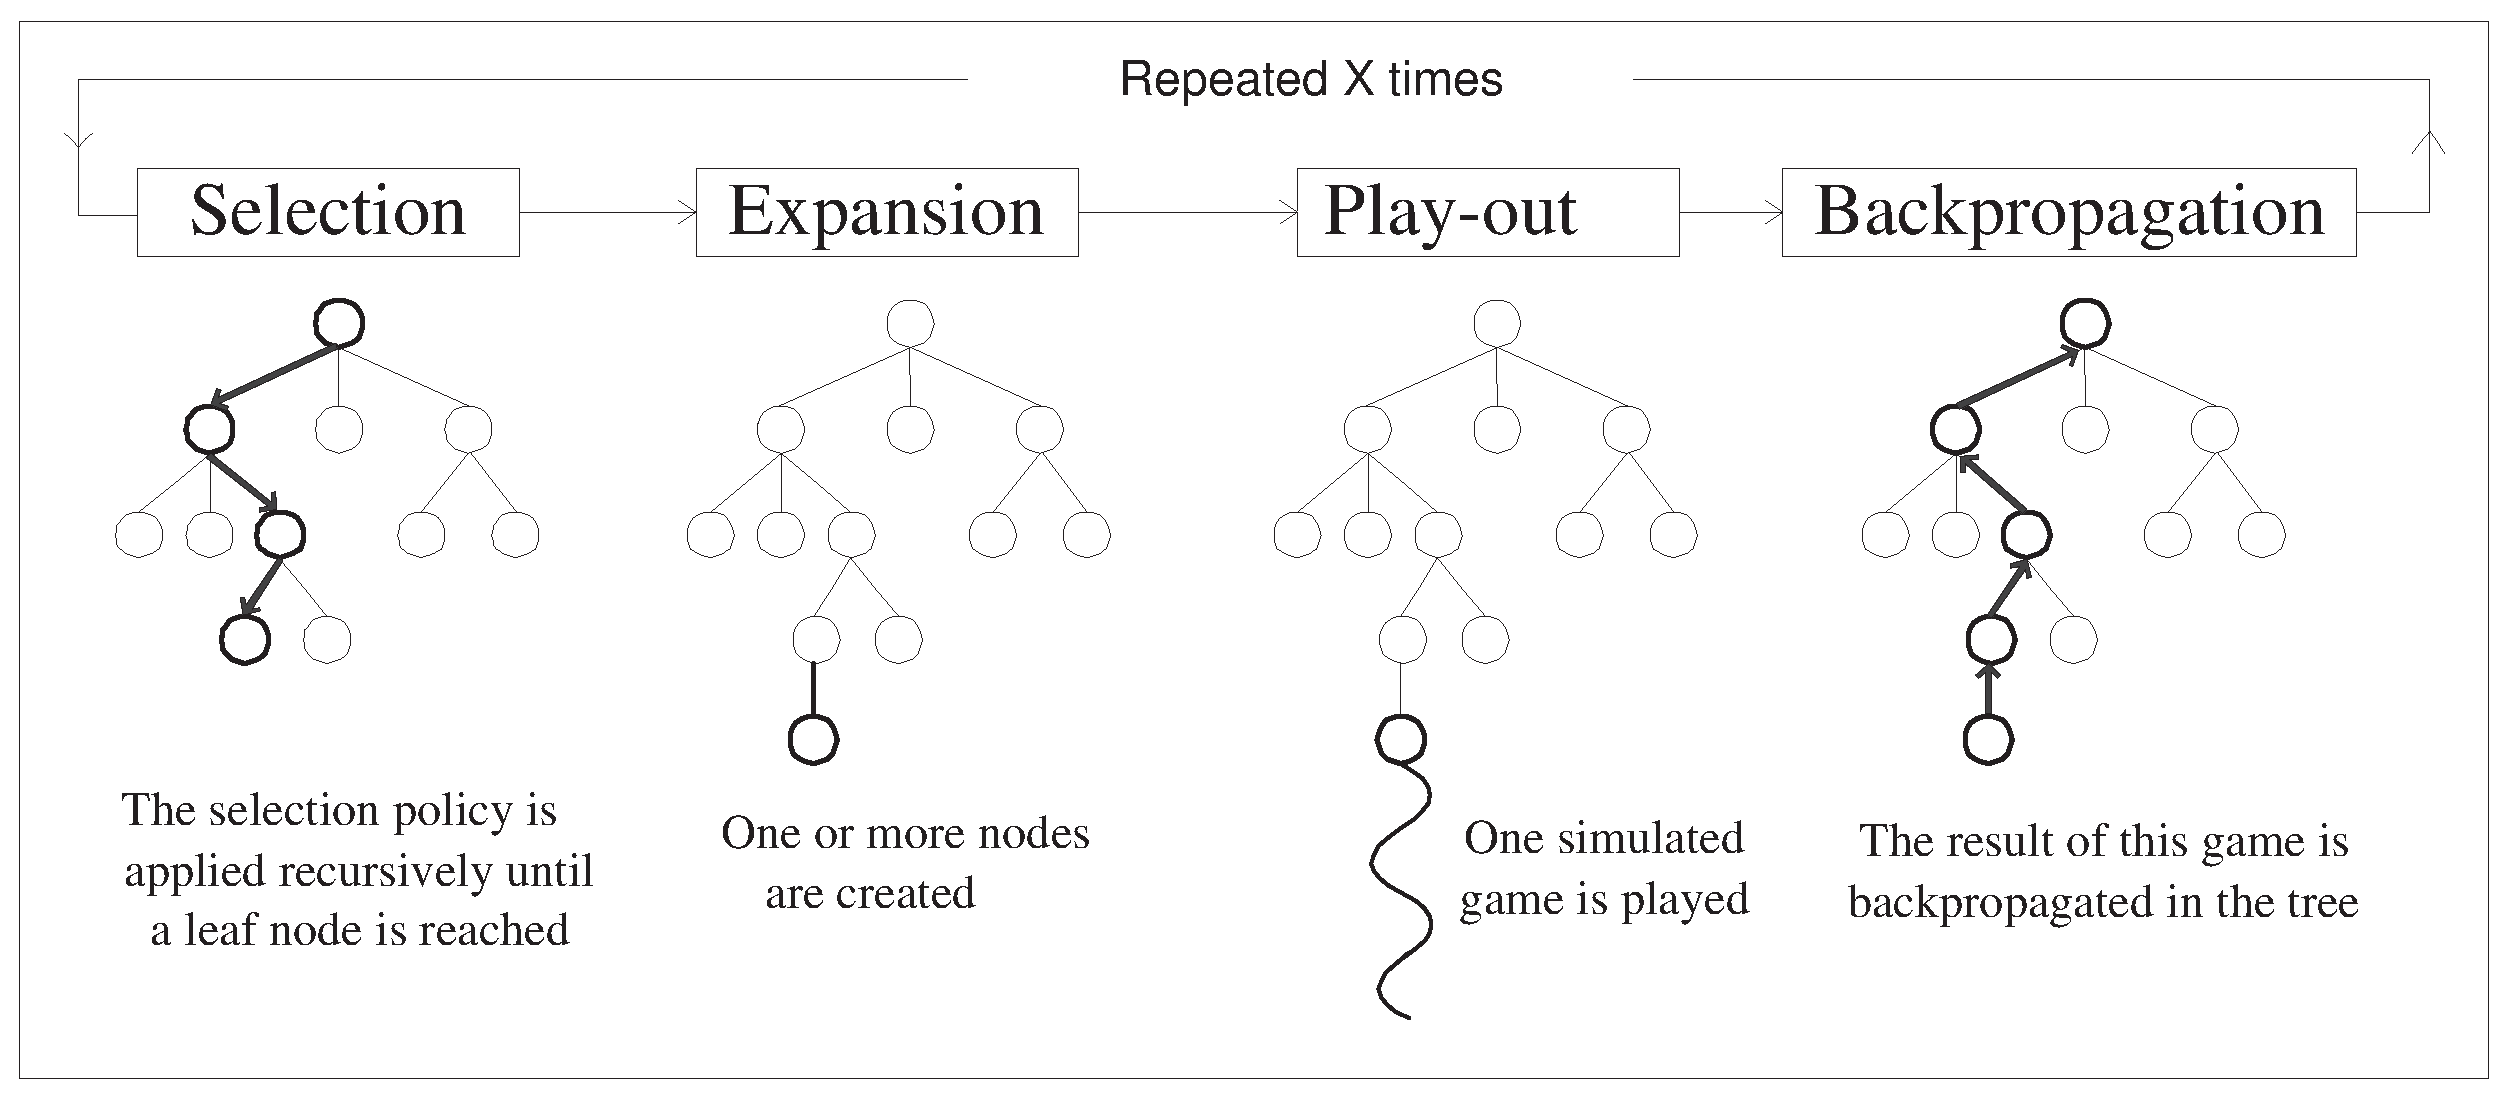
\includegraphics[width=1.\textwidth]{img/figure1.eps}
	\caption{Strategic steps of Monte-Carlo Tree Search~\protect\citebay{chaslot2008progressive}.}
	\label{fig:mcts-algorithm}
\end{figure}
\noindent In MCTS, a tree is built incrementally over time, which maintains statistics at each node corresponding to the rewards collected at those nodes and number of times  they have been visited. The root of this tree corresponds to the current position. When using a bandit-based method to select moves, such as in UCT, MCTS resembles a recursive multi-armed bandit. The basic version of MCTS consists of four steps, which are performed iteratively until a computational threshold is reached, \ie a set number of iterations, an upper limit on memory usage, or a time constraint. The basic version of MCTS consists of four steps \citebay{chaslot2008progressive}:
\begin{itemize}
\item {\bf Selection}. Starting at the root node, children are selected recursively according to a selection policy. When a leaf node is reached that does not represent a terminal state it is selected for expansion.
\item {\bf Expansion}. All children are added to the selected leaf node given available moves.
\item {\bf Play-out}. A simulated play-out is performed, starting from the state of the added node. Moves are performed randomly or according to a heuristic strategy until a terminal state is reached.
\item {\bf Back-propagation}. The result of the simulated play-out is propagated immediately from the selected node back up to the root node. Statistics are updated along the tree for each node selected during the selection phase and visit counts are increased.
\end{itemize}
The combination of moves selected during the selection step, and the play-out form a single simulation. During the selection step, moves are executed according to the nodes selected in the tree, and during play-out moves are performed randomly, or according to some play-out policy.

Because results are immediately back-propagated, MCTS can be terminated any time to determine the decision to be made. Moreover, no static heuristic evaluation is required when simulations reach an end state. However, in most cases it is beneficial to add domain knowledge for choosing moves made during the play-out.

The main benefit of MCTS is that it requires no explicit heuristic state evaluation. Rather, states are evaluated by repeatedly sampling them and measuring an average reward. That being said, it is often beneficial to add some domain knowledge to the play-outs such that the simulated games better approximate good play. Moreover, many enhancements to MCTS have been proposed to improve the general performance of the algorithm. Most notably, the MCTS-Solver \citebay{Winands2008} recognises solved wins and losses in the tree and backpropagates their values, RAVE~\citebay{gelly2007} used to speed up node valuation in the tree, and simulation-policy learning techniques such as low-level $\alpha\beta$ searches~\citebay{Winands2011}, and methods that learn a strategy online, such as the Last-Good-Reply policy~\citebay{baier2010power}, Move-average Sampling Technique (MAST)~\citebay{finnsson2008simulation}, or N-Grams~\citebay{Tak2012}. Combining these techniques often offers greatly improved play by MCTS.

\section{Regret Minimization}
The driving force behind MCTS is the notion of regret minimization. Algorithms used in multi-armed bandit research have been developed to minimize \emph{cumulative regret}. Cumulative regret is the expected regret of not having sampled the optimal decision. This type of regret is accumulated during execution of the algorithm, each time a non-optimal arm is sampled the cumulative regret increases. UCB1~\citebay{auer2002using} is a selection policy for the MAB problem, which minimizes cumulative regret at a fast rate, converging to the empirically best arm fast. Once the best arm is found by exploring the available options, UCB1 exploits it by repeated sampling, minimizing overall cumulative regret. This policy was adapted to be used in MCTS in the form of UCT~\citebay{kocsis2006bandit}

Recently, \emph{simple regret} has been proposed as a new criterion for assessing the performance of both MAB~\citebay{audibert2010best,Bubeck11Pure} and MCTS~\citebay{tolpin2012mcts,Feldman12BRUE,Cazenave14SHOT} algorithms. Simple regret is defined as the expected error between an algorithm's recommendation, and the optimal decision. A naturally fitting quantity to optimize in the MCTS setting, since all simulations executed by MCTS are for the mere purpose of learning good moves. However, the final move chosen after all simulations are performed, \ie the \emph{recommendation}, is the one that has real consequence. Therefore, the choice of this move should have as low as possible simple regret. Moreover, once MCTS finds a good move with high certainty, the utility of re-selecting that move diminishes over time. When a promising node, or group of nodes is visited too often, at a certain point insufficient simulation time remains to determine whether there exists a viable alternative. Rather it may be favourable to explore other options sooner, even if a single move is identified as the best. At the same time, MCTS should not `waste' its time on moves that are expected to be bad.

This is the driving idea behind pure exploration algorithms such as Successive Rejects~\citebay{audibert2010best} and Sequential Halving~\citebay{Karnin13SH}. Contrary to UCB, these algorithms have no specific exploitation phase, they divide their time uniformly between a continuously reduced set of options. The final recommendation is the single arm that remains after all trials are finished.
\newpage
\section{Problem Statement and Research Questions}
When MCTS is applied to games it is only the final recommendation, \ie the actual move played, that has an impact. To this end, we want the probability of selecting a suboptimal move, \ie the expected simple regret, to be as low as possible. Based on this assumption, simple regret minimization can be a better way to determine a move's utility. As such, a method that minimizes both types of regret in their appropriate settings can improve the overall performance of MCTS. Simple regret optimization (pure exploration) has practical problems, especially at low search times because it spends more time on sub-optimal decisions than UCT. Whereas techniques based on cumulative regret perform particularly well under such limited circumstances. Currently several algorithms have been proposed to minimize simple regret. However, some do not improve performance in games, while others only provide benefits in specific circumstances.

The problem statement of this thesis is:
\newline \newline
\emph{How can a Monte-Carlo Tree Search variant be constructed that minimizes both simple and cumulative regret effectively?}
\newline \newline
The following four research questions arise from this problem statement:
\begin{enumerate}

\item{\emph{How can a search technique be developed for minimizing both simple and cumulative regret in a game tree?}}
\item{\emph{At which point should the selection policy switch from simple to cumulative regret minimization in the tree?}}
\newline
\NoIndent{To answer these questions, an investigation into state-of-the-art multi-armed bandit algorithms is required. Additionally, some MCTS variants already minimize simple regret, such as SHOT~\citebay{Cazenave14SHOT} and a technique that minimizes simple regret only at the root~\citebay{tolpin2012mcts}. These algorithms provide the inspiration and technique for a new Hybrid MCTS (H-MCTS).
Given the new Hybrid technique, our initial assumption regarding simple regret minimization in games ought to be verified:}

\item{\emph{Does using simple regret minimizing, pure exploration selection policies in MCTS improve performance in two-player games?}}
\newline
\NoIndent{This question is answered by performing experiments in six distinct two-player games: Amazons, AtariGo, Ataxx, Breakthrough, NoGo, and Pentalath. For which, H-MCTS' performance is compared to both UCT and SHOT. The last research question relates to an existing MCTS enhancement:}

\item{\emph{How can the MCTS-Solver by~\citeaby{Winands2008}, be adapted to work with the new MCTS technique?}}
\newline
\NoIndent{To address the last research question, the MCTS-Solver is adapted and implemented in the new technique.}
\end{enumerate}

\section{Thesis Outline}

The thesis opens with two introductory chapters introducing and discussing the background of the theory used. \textbf{Chapter \ref{chap:mab}}, which discusses the Multi-armed Bandit problem and its application to MCTS, and \textbf{Chapter \ref{chap:mctssr}}, in which current simple regret minimizing MCTS algorithms are discussed. The former details the exact difference between simple and cumulative regret, and how these types of regret may be minimized using different selection policies, and the latter shows how these selection policies are applied to MCTS.

Next, \textbf{Chapter \ref{chap:hybmcts}} goes into detail on Hybrid MCTS. Based on the analysis in the previous chapters, the new algorithm is defined and described. Moreover, the problems and shortcomings of the algorithm are discussed, and possible solutions provided. In \textbf{Chapter \ref{chap:experiments}} the proposed algorithm is tested in six two-player games: Amazons, Breakthrough, AtariGo, Ataxx, and Pentalath. \textbf{Chapter \ref{chap:conclusion}} concludes the thesis, and offers directions for future research and improvements.

% --------------------------------------------------------------------------------------
% ------------------- ::::::: Regret And Multi-Armed Bandits ::::::: -------------------
% --------------------------------------------------------------------------------------
\chapter{Regret And Multi-Armed Bandits}
\label{chap:mab}
\begin{chaptercontents} The foundation of regret minimization for Monte-Carlo Tree Search (MCTS) is given. Given that UCT is defined a recursive Multi-Armed Bandit algorithm, regret minimization is discussed in this context first. Two algorithms designed to minimize simple regret in Multi-Armed Bandits are outlined. Moreover, the link between simple and cumulative regret is detailed and recent findings are discussed. 
\end{chaptercontents}

\section{Introduction}
The Multi-Armed Bandit problem is defined as a stochastic decision making problem~\citebay{Robbins_someaspects}. An agent is faced with several options, each with their own reward distribution. Based on sampling the search space an agent is to select the option with the best reward distribution. Generally the problem is described as choosing between the most rewarding arm of a multi-armed slot machine found in casinos. The agent can explore by pulling an arm and observing the resulting reward. The reward is drawn from either a fixed or changing probability distribution. Each pull and the returned reward constitutes a sample.

In the classic MAB setting, the goal is to maximize the cumulative sum of rewards, \eg winning the most money in the slot machine example. Since the agent does not know the distribution of the arms beforehand, he has to \emph{explore} the possible choices, and when a rewarding arm is found, \emph{exploit} this option to gain a high total reward. Generally, after a certain limit, \eg a time-span or number of trials, the agent must return a recommendation to determine the best arm.

The performance of the agent can be evaluated by observing the difference in the rewards obtained over time and the theoretical reward obtained by pulling only the true best arm, called \emph{cumulative regret}. Or, in the case of \emph{simple regret}, observing the difference between the recommended arm and the true best arm, after the forecaster makes its final recommendation.
\vspace{2 mm}

In this chapter the different facets of the MAB problem are discussed and related to MCTS. In Section \ref{sec:mabprob} a formal definition of the two types of regret, and their interrelation is given. Next, Section \ref{sec:ucb} discusses the well-known UCB1 selection policy and its relation to MCTS. This is followed by a review of two recently introduced selection policies for MAB aimed at minimizing simple regret, in Section \ref{sec:pureexplmab}.

\newpage

\section{Regret and The Multi-Armed Bandit Problem}
\label{sec:mabprob}
Suppose a trial is set-up such that a forecaster (a player, or agent) has $i \in [[K]] = \{1, 2, \cdots, K \}$ actions, which can be repeatedly sampled over $n \in \{ 1, 2, \cdots, T \}$ trials. Each arm has a mean reward $\mu_i$, and there exists an optimal mean reward $\mu^*$. Suppose further that the forecaster employs a selection policy $I(n)$ that outputs some $a$ to be sampled at time $n$, and a recommendation policy $J(n)$ that selects the best arm at $T$.

\emph{Cumulative regret} is defined as the regret of having not sampled the best single action in hindsight, 
\begin{equation}
R_n = \sum_{t = 1}^{n}{\mu^* - \mu_{I(t)}}.
\end{equation}
In other words, the regret is accumulated over time, for each sample the forecaster takes.

Now suppose that we change the experimental set-up, such that the actions chosen on trials $1, 2, \ldots, T-1$ are taken under some realistic ``simulated environment'' that represents the true on-line decision problem but without committing to the actions. The only \emph{real} decision is made at step $T$ after having played $T-1$ simulations. In contrast, \emph{simple regret}~\citebay{Bubeck11Pure} quantifies only the regret for the recommendation policy $J$ at time $T$,

\begin{equation}
r_n = \mu^* - \mu_{J(n)},
\end{equation}
\ie the regret of not having recommended the best action.

Given these definitions, a performance metric for a selection technique can be described as the expected cumulative $\bE R_n$ or simple regret $\bE r_n$ over different experiments. In their analysis of the links between simple and cumulative regret~\citeaby{Bubeck11Pure} found that upper bounds on $\bE R_n$ lead to lower bounds on $\bE r_n$, and that the smaller the upper bound on $\bE R_n$, the higher the lower the lower bound on $\bE r_n$, regardless of the recommendation policy, \ie the smaller the cumulative regret, the larger the simple regret. As such, no policy can give an optimal guarantee on both simple and cumulative regret at the same time. In the case of a multi-armed bandit the strategy used depends on the context of the problem.

\section{UCB}
\label{sec:ucb}

\citeaby{auer2002using} proposed a finite time strategy for the multi-armed bandit problem. UCB1 optimizes cumulative regret over time at an optimal logarithmic rate, without knowledge of the reward distributions. The selection policy consists of two terms, 1) the current average reward, and 2) the size of the one-sided confidence interval for the average reward. For each arm, UCB1 gives an upper bounding value, below which, the true expected reward of the arm falls with high probability. The UCB1 selection policy is outlined in Algorithm \ref{alg:ucb}.

\IncMargin{1em}
\RestyleAlgo{boxruled}
\begin{algorithm2e}[ht]
	\Indm
	\KwIn{total budget $T$, arms $K$}
	\KwOut{recommendation $J_T\in [[K]]$}
	\vspace{0.2cm}
	\Indp

	play each arm once 																				\;

	\For{t=1 \emph{\KwTo} $T$} {
		Sample arm $i$ that maximizes $\bar{x}_i + \displaystyle\sqrt{\frac{2\ln{t}}{n_i}}$ \newline
		$\bar{x}_i$ is the current average reward of arm $i$, $n_i$ is the total number of samples for arm $i$ \;
	}

	\KwRet{the element of $K$ with the highest average reward}
  \caption[Upper Confidence Bounds (UCB1)]{Upper Confidence Bounds (UCB1)~\protect\citebay{auer2002using}. \label{alg:ucb}}
\end{algorithm2e}
\DecMargin{1em}

The rate of growth of cumulative regret of UCB1 is $\ln(n)$, where $n$ is the number of samples, which was shown to be the optimal rate by~\citebay{lai1985asymptotically}. \citeaby{Bubeck11Pure} show that a recommendation based on such a selection policy suffers a simple regret that decreases at best at a polynomial rate. 

Later in this chapter, in Section \ref{sec:mabmcts} UCB1 is discussed in the context of MCTS. Where its adopted version UCT, is widely used as the preferred selection policy.
\newpage
\section{Pure Exploration in Multi-Armed Bandits}
\label{sec:pureexplmab}
Non-exploiting selection policies have been proposed to decrease simple regret at high rates. Given that UCB1 has an optimal rate of cumulative regret convergence, and the conflicting limits on the bounds on the regret types shown by~\citeaby{Bubeck11Pure}, policies that have a higher rate of exploration than UCB1 has better bounds on simple regret. 

Consider a uniform selection policy that samples each arm of an MAB $T/K$ times. Assuming that there are $h$ best arms, $(K-h)T/K$ trials are spent sampling inferior arms, and $hT/K$ on the best one(s). Such a selection policy has simple regret $\bE r_n = \bE R_n/n$.
In games, there are often only one or two good moves to be identified, and therefore when using uniform selection, most time is spent sampling suboptimal arms. Therefore, a more efficient policy is required to ensure that inferior arms are not selected as often as arms with a high utility over time. Two algorithms, discussed in this section, have been proposed to solve this problem.

Both algorithms have shown to outperform the other in different problem settings~\citebay{Karnin13SH}. Sequential Halving gives better results when there are multiple groups of suboptimal arms, or when the arm's rewards form an arithmetic or geometric series. Successive Rejects performs best when there is a single group of suboptimal arms, or when selecting over a small subset of arms. Both methods have proven theoretical guarantees with regard to the simple regret bounds, and a near-optimal, exponential rate of decrease on simple regret. Based on this it holds merit to consider these algorithms as candidate substitutes for UCT in MCTS. However, based on the analysis made by~\citebay{Bubeck11Pure} discussed in Section \ref{sec:mabprob}, any method that effectively minimizes simple regret has inferior bounds on its cumulative regret. Therefore, there may be some trade-off between using pure exploration methods and UCT.
\newpage
\subsection{Successive Rejects}
\IncMargin{1em}
\RestyleAlgo{boxruled}
\begin{algorithm2e}[ht]
	\Indm
	\KwIn{total budget $T$, arms $K$}
	\KwOut{recommendation $J_T\in [[K]]$}
	\vspace{0.2cm}
	\Indp
	$S_1 \gets \{1,\dots,K\}$, $n_0 \gets 0$										\; 
	$\widebar{log}(K) \gets \frac{1}{2} + \sum_{i=2}^{|K|} \frac{1}{i}$				\;
	\BlankLine
	\ForEach{$k\in\{1,\dots,K-1\}$} {
		$n_k = \displaystyle\ceil[\bigg]{\frac{1}{\widebar{log}(K)} \frac{T-|K|}{|K|+1-k}}$				\;
	}
	\BlankLine
	\For{k=1 \emph{\KwTo} $|K|-1$}{
		Sample each arm $i\in S_k$ $n_k - n_{k-1}$ times 						\;	\label{succrej:subtr}
		$S_{k+1} \gets$ the $|S_k|-1$ empirically best arms from $S_k$			\;
	}
	\BlankLine
	\KwRet{the single element of $S_K$}
  \caption[Successive Rejects]{Successive Rejects~\protect\citebay{audibert2010best}. \label{alg:succrej}}
\end{algorithm2e}
\DecMargin{1em}

Successive Rejects~\citebay{audibert2010best} works by successively removing the single worst arm from the selection. The algorithm computes a budget for each round $n_k$, during the round, each arm is selected an equal number of times. After each round, the empirically worst arm is removed from the selection and a new round started. The lengths of the rounds are computed in such a manner that a specific lower bound on simple regret is guaranteed.

Successive Rejects is detailed in Algorithm~\ref{alg:succrej}. Note that, since $n_0 = 0$ the algorithm starts with a relatively long initial round. Followed by the shortest round, due to the subtraction on line \ref{succrej:subtr}. However, the length of the rounds increases when more arms are removed. An example run is depicted in figure \ref{fig:succ-rej}, where a total budget $T = 200$ is allocated to 5 arms, the number of samples per arm for each round is shown. For the first round the trials per arm are $\ceil{\frac{60}{107} \frac{200-5}{5+1-1}} - 0 = 22$ subsequently, for the second round $\ceil{\frac{60}{107} \frac{200-5}{5+1-2}} - 22 = 6$ and so on. The recommended arm is sampled a total of $57$ times.

\begin{figure}[ht]
	\centering
	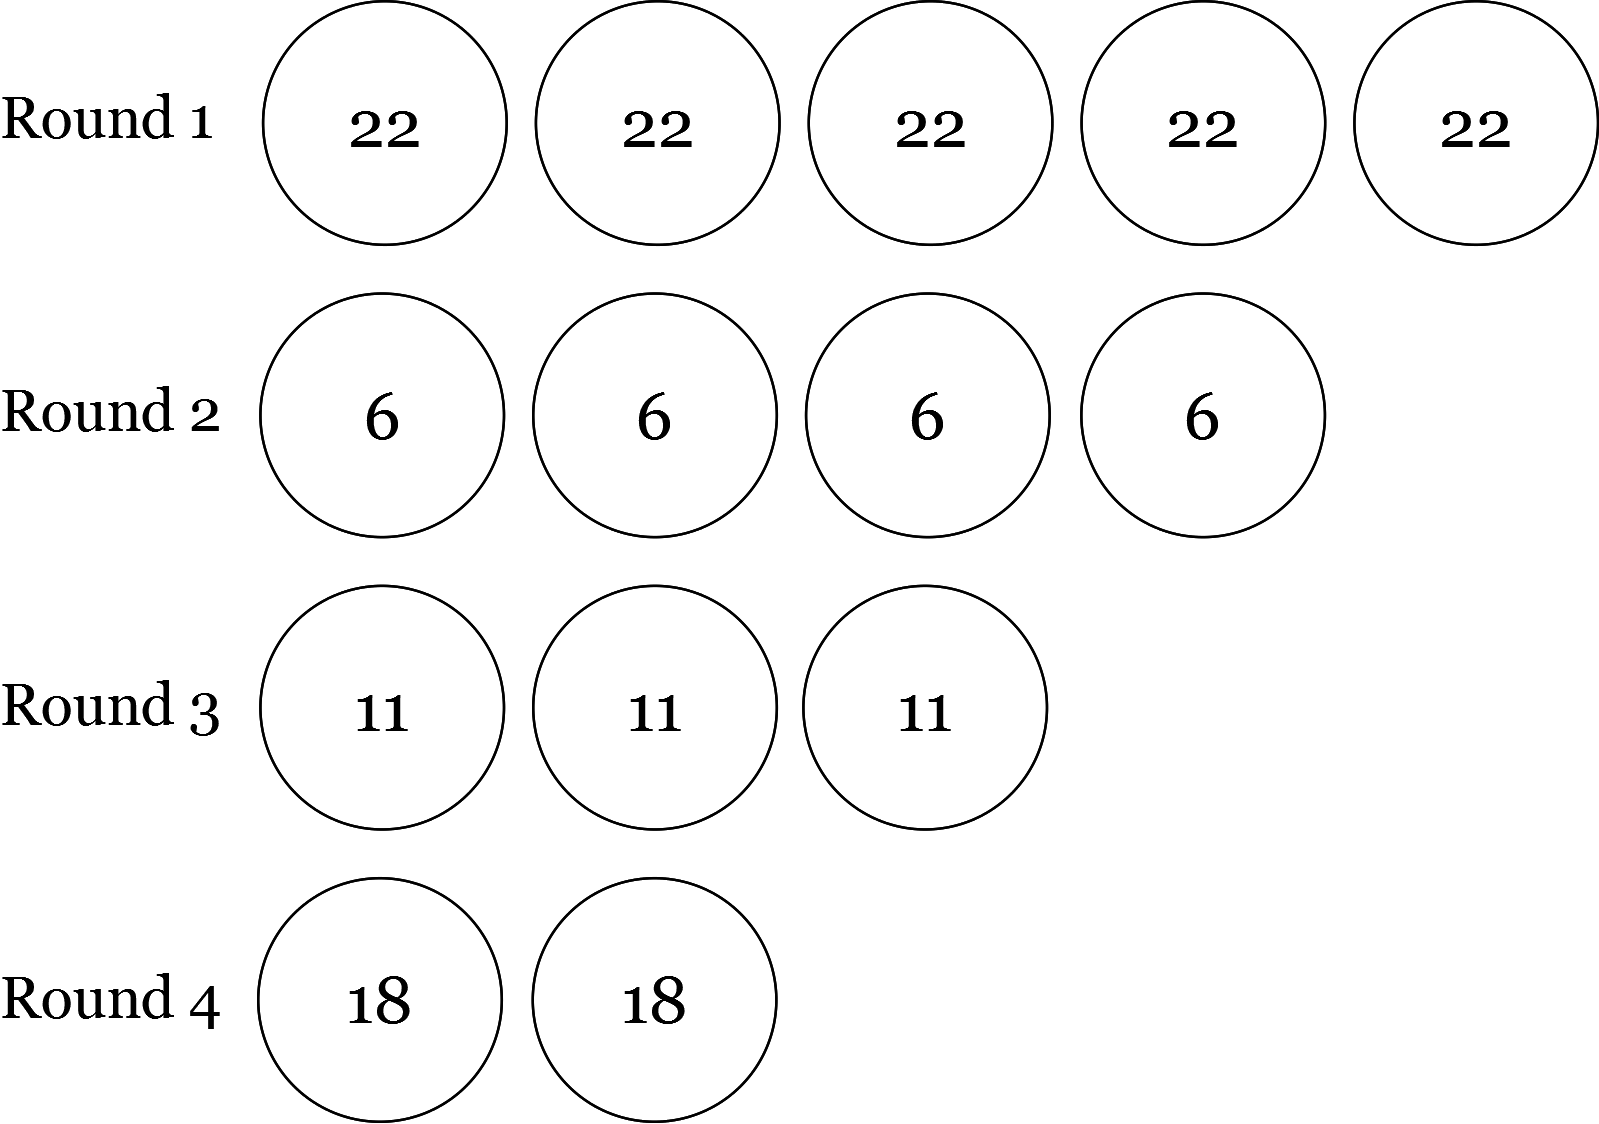
\includegraphics[width=.6\textwidth]{img/succ_rej.png}
	\caption{Successive Rejects example on 5 arms and a total budget of 200.}
	\label{fig:succ-rej}
\end{figure}

\newpage

\subsection{Sequential Halving}
Sequential Halving~\citebay{Karnin13SH} takes an approach similar to Successive Rejects. As with Successive Rejects, search time is divided into rounds, and during each round arms are sampled uniformly. However, instead of removing a single arm from selection after each round, half the arms are removed until a single one remains. The rounds in Sequential Halving are equally distributed such that constitute the same number of trials, but with a decreased subset of arms to select. Sequential Halving is detailed in Algorithm~\ref{alg:seqhalv}.

\IncMargin{1em}
\begin{algorithm2e}[ht]
\setstretch{1.1}
	\KwIn{total budget $T$, arms $K$}
	\KwOut{recommendation $J_T\in [[K]]$}
	\vspace{0.1cm}
	$S_0 \gets \{1,\dots,K\}$,
	$B \gets \ceil{\log_2{|S|}} - 1$														\;
	\BlankLine
	\For{k=0 \emph{\KwTo} $B$}{
		sample each arm $i \in S_k$, 										
		$n_k = \floor[\bigg]{\frac{T}{|S_k|\ceil{\log_2{|S|}}}}$
		times 																				\;
		\vspace{0.1cm}
		$S_{k+1} \gets$ the $\ceil{|S_k|/2}$ arms from $S_k$ with the best average			\;
	}
	\KwRet{the single element of $S_k$}
  \caption[Sequential Halving]{Sequential Halving~\protect\citebay{Karnin13SH}. \label{alg:seqhalv}}
\end{algorithm2e}
\DecMargin{1em}

An example of the budget allocation by Sequential Halving is depicted in Figure \ref{fig:seq-halving}, where a total budget $T = 200$ is allocated to $5$ arms, the allocated budget per arm for each round is shown. At time $T$, after $\ceil{\log_2{5}}=3$ rounds, the single remaining arm is recommended. This arm is sampled $68$ times, $11$ times more than the recommended arm in the same example given for Successive Rejects.

\begin{figure}[ht]
	\centering
	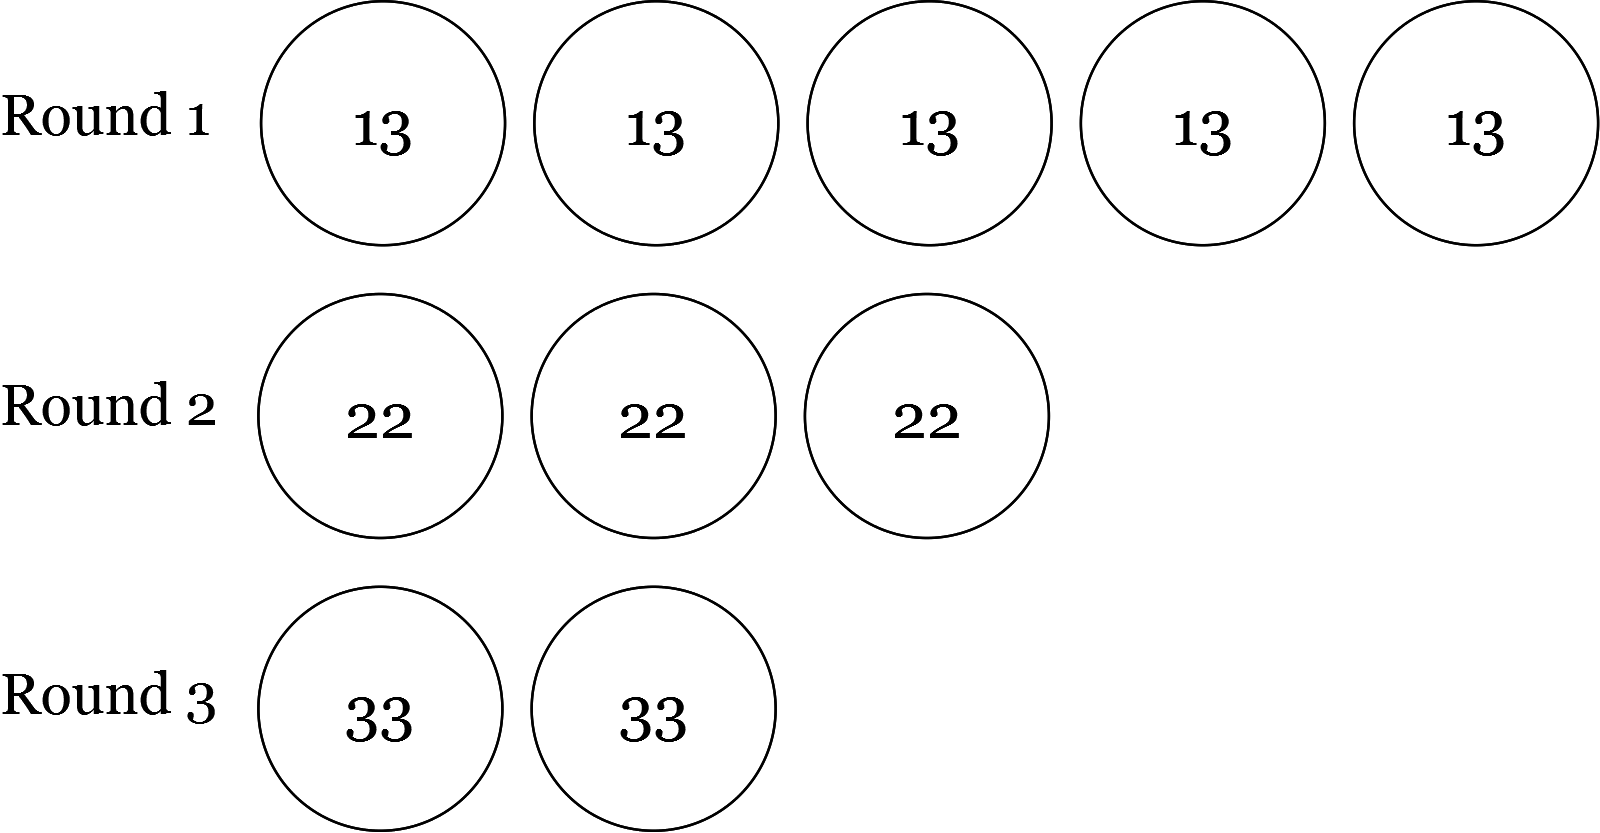
\includegraphics[width=.6\textwidth]{img/seq_halving.png}
	\caption{Sequential Halving example on 5 arms and a total budget of 200.}
	\label{fig:seq-halving}
\end{figure}

Sequential Halving is a candidate for a recursive definition to be used in MCTS. The algorithm performs well in the cases described in the original article, samples the best node more frequently than Successive Rejects, and the budget per round is easily calculated. An MCTS variant that implements Sequential Halving recursively named SHOT~\citebay{Cazenave14SHOT}, is discussed in Chapter~\ref{chap:mctssr}

\newpage

\section{Relation to MCTS}
\label{sec:mabmcts}
\subsection{UCT}
During the MCTS selection step, a policy is required to explore the tree to decide on promising options. For this reason, the widely used Upper Confidence Bound applied to Trees (UCT)~\citebay{kocsis2006bandit} was derived from the UCB1 policy. In UCT, each node is treated as a bandit problem whose arms are the moves that lead to different child nodes. UCT balances the exploitation of rewarding nodes whilst allowing exploration of lesser visited nodes. Consider a node $p$ with children $I(p)$, then the policy determining which child $i$ to select is defined as:

\begin{equation}
\label{eq:uct}
i^* = argmax_{i \in I(p)}\left\{ v_i + C \sqrt{ \frac{\ln{n_p}}{n_i}}\right\},
\end{equation}
where $v_i$ is the score of the child $i$ based on the average result of simulations that visited it, $n_p$ and $n_i$ are the visit counts of the current node and its child, respectively. $C$ is the exploration constant to tune. UCT is applied when the visit count of a child node is above a threshold $T$. When a node's visit count is below this threshold, a child is selected at random.

Note that, UCB1 and, consequently UCT incorporates both exploitation and exploration. After a number of trials, a node that is identified as the empirical best is selected more often. In tree search, this has three consequences:
\begin{enumerate} 
\item Whenever a promising move is found, less time is spent on suboptimal ones. Since UCT is generally time-bounded, it is important to spend as much time as possible exploiting the best moves. Because, by the \emph{MinMax} principle, on each ply we expect a player to maximize his minimum gain. 

\item The valuation of any node in the tree is dependent on the values back-propagated. Given that UCT spends less time on suboptimal moves, any values back-propagated are based on increasingly better approximations of simulations performed deeper in the tree. In fact, given infinite time, UCT converges to selecting only moves with the highest average values.

\item The current value of the node can be falsified by searching deeper. In UCT, each simulation increases the depth of the search, and as such may reveal moves as becoming worse over time due to an unpredicted turn of events. If an expected good move is not reselected often, such ``traps''~\citebay{Ramanujan2010a} are not revealed.
\end{enumerate}

\subsection{Regret in MCTS}

Based on the analysis in the previous subsection, the minimization of cumulative regret is naturally suitable to tree search, and the UCB1 selection policy can be used nearly unaltered in this setting as UCT. However, as is shown in Section \ref{sec:mabprob} there exist two contexts for the multi-armed bandit problem, also to be considered in MCTS. These are:

\begin{enumerate}

\item Each trial results in a direct reward for the agent. As such we want to minimize the number of suboptimal arms pulled in order to achieve an as high as possible reward. This relates, for example, to slot machines in a casino. Every choice made at each point in the algorithm has a direct effect on the agent's reward. In this case, the reward of the agent is inversely proportional to its \textbf{cumulative regret}.

\item The agent can perform a number of trials, without consequence, in a simulated environment. The agent is allowed $T$ trials in this fashion, after which it must make a recommendation. Based on its recommendation, the agent is rewarded. In this case, the performance of the agent is measured by the \textbf{simple regret} of its recommendation. A low simple regret implies that the recommendation is close to the actual best option.

\end{enumerate}

In most MCTS literature, UCT is used as selection policy~(\cf~\citebay{browne2012survey}), suggesting that the first context applies. However, the second context is a more natural fit when MCTS is used to play games, because the behavior of the agent in the domain is based solely on its recommendations. Nevertheless, simple regret minimization cannot replace UCT in this case without consideration. Unlike in an MAB, sampling does have an immediate impact on performance in MCTS because reward distributions are non-stationary. 
However, simulations in MCTS do have an immediate impact on its performance. First of all, since MCTS must make a recommendation in a finite amount of time, spending more time on sub-optimal moves decreases time available to explore those expected to have high utility. This was also shown in~\citebay{tolpin2012mcts} where the authors used a measure based on the Value of Information (VOI) to determine whether to exploit an expected good move. This trade-off is also described as a ``separation of exploratory concerns'' in BRUE~\citeaby{Feldman12BRUE}.

The general performance of MCTS may be improved by applying a strategy that is focused on minimizing simple regret fast, rather than cumulative regret, in some specific part of a search-tree. Given that simple regret is a better measure of the quality of a given decision at time $T$, and that we can apply both the aforementioned contexts to search in a specific manner. 

In the next chapter, MCTS variants designed to (partially) minimize simple regret are discussed. Subsequently, in Chapter~\ref{chap:hybmcts}, a new search technique is proposed that uses both simple and cumulative regret minimizing policies at appropriate segments of the MCTS tree. Using this technique, we can determine whether the assumption that, when using a recursive multi-armed bandit algorithm such as MCTS in games, preferring simple over cumulative regret minimization is both practical, and improves overall performance.

% -----------------------------------------------------------------------------
% ------------------- ::::::: Simple Regret In MCTS ::::::: -------------------
% -----------------------------------------------------------------------------
\chapter{Simple Regret In MCTS}
\label{chap:mctssr}

\begin{chaptercontents} A discussion on MCTS variants using simple regret minimizing selection policies. This chapter serves as introduction and inspiration to the next in which the new search technique, which combines different selection policies, is detailed.
\end{chaptercontents}

\section{Introduction}
Since the introduction of MCTS~\citebay{kocsis2006bandit} and its subsequent adoption by games researchers~(\cf~\citeaby{browne2012survey}) UCT, or some variant thereof, has become the ``default'' selection policy. Since the introduction of simple regret~\citebay{Bubeck11Pure}, more MCTS research has been performed using simple regret as the minimizing metric.

\citeaby{Feldman12BRUE} have proposed an algorithm named {\sc brue}, devoted to offering the low simple regret bounds. Rather than building a connected tree such as MCTS, {\sc brue} generates non-connected nodes based on a switching function. The authors mention that the algorithm is a possible replacement for UCT. In \citeaby{Feldman13}, {\sc brue} is extended such that it may be used in more practical domains. Importantly, the proposed {\sc brue\textsubscript{i}} can be used without specifying a fixed horizon, rather it builds a tree connected to the root incrementally. Based on experimentation with {\sc brue} and {\sc brue\textsubscript{i}} in the games discussed in this thesis, no improvement was shown over UCT. Based on this, the algorithm is not discussed in this chapter.

Rather than optimizing either simple, or cumulative regret throughout the MCTS tree,~\citeaby{tolpin2012mcts} propose a technique in which simple regret is minimized only at the root. As is the case with {\sc brue}, the authors developed this algorithm for solving \emph{Markov decision processes}. SHOT~\citebay{Cazenave14SHOT} is an MCTS algorithm based on sequential-halving~\citebay{Karnin13SH}. This algorithm was developed to provide a speed-improvement over UCT, allowing more simulations per second to be performed and thereby increasing performance in game-play. 

\vspace{2 mm}
The proposed techniques are discussed in this chapter, because their approaches lead to key insights for the development of a hybrid MCTS. In this chapter two MCTS variants are discussed. First, in Section \ref{sec:srmcts}, the so-called (SR+CR) scheme proposed by~\citebay{tolpin2012mcts} is discussed. Next, in Section \ref{sec:SHOT}, a recently introduced algorithm, SHOT~\citebay{Cazenave14SHOT} is detailed. Both algorithms form the foundation of Hybrid MCTS, which is introduced in the next chapter.
\newpage
\section{MCTS Based on Simple Regret}
\label{sec:srmcts}

\citeaby{tolpin2012mcts} give the same arguments presented in Chapter \ref{chap:mab}, that when MCTS is used in a the context of search in an MDP, \emph{``it is usually only the final ``arm pull'' (the actual move selection) that collects a reward, rather than all ``arm pulls''''}~\citebay{tolpin2012mcts}. Moreover, the exploitation of high valued nodes is not preferable in all circumstances. Rather, more time should be spent exploring the alternatives. The hypothesis of the article is that, since only the children of the root represent an action to be taken in the domain, a selection policy that minimizes simple regret at the root, and UCT throughout the rest of the tree, should have better performance than using only UCT.

Two selection policies with lower bounds than UCT on simple regret were constructed for the purpose of selecting nodes at the root.
\begin{enumerate}
\item $\frac{1}{2}$-greedy, a policy that selects a move at random half of the time, and the current empirical best the other half. This policy offers an exponentially decreasing simple regret.
\item ${UCB}_{\sqrt{.}}$, which is similar to UCT, however the logarithm in the numerator in the upper confidence bound is replaced by a square root.
\begin{equation}
\label{eq:uctsqrt}
i^* = argmax_{i \in I(p)}\left\{ v_i + C \sqrt{ \frac{\sqrt{n_p}}{n_i}}\right\}
\end{equation}
This selection policy has a super-polynomially decreasing simple regret.
\end{enumerate}

Next, a two-stage sampling scheme named {\sc sr+cr} uses one of the above policies at the root, and UCT in the rest of the tree. In Algorithm \ref{alg:tsmcts}, the scheme proposed by the authors is given in the context of game-play.
\IncMargin{1em}
\RestyleAlgo{boxruled}
\begin{algorithm2e}[ht]
\setstretch{1.2}
	\KwIn{node $p$, current search depth}													
	\func{srcr-mcts}(node $p$, $depth = 1$):														\;
	\Indp							
	\lIf{isLeaf($p$)}{Expand($p$)}
	\eIf{$depth = 1$} {
	select child $i$ using $\frac{1}{2}$-greedy or ${UCB}_{\sqrt{.}}$								\;
	}
	{
	select child $i$ using UCT 																		\;
	}

    \eIf{isLeaf(i)} {
    	$r \gets$ {\sc playout}$(i)$ 																\;
    	\func{update} node $i$ with $r$																\;
    }
    {
    	$r \gets$ -\func{srcr-mcts}($i$, $depth + 1$)												\;
    }	
    \func{update} node $p$ with $r$																	\;
	\Indm
    \KwRet{$r$}
  \caption[Two-stage Monte-Carlo Tree Search]{Two-stage Monte-Carlo Tree Search~\protect\citebay{tolpin2012mcts}. \label{alg:tsmcts}}
\end{algorithm2e}
\DecMargin{1em}

The selection policies were empirically validated to have lower simple regret than UCB in multi-armed bandits. Moreover, the {\sc sr+cr} scheme was shown to have lower simple regret in the MDP sailing domain. Particularly, the scheme was more advantageous when the number of nodes at the root are higher.

Although the {\sc sr+cr} scheme and two-stage MCTS was not developed for game-play, it holds merit to attempt to replicate the favourable results presented in games. Since, as the authors argue, only the options given at the root collect any true reward from the domain, and this is the case in both MDP domains and games. The algorithm presented was implemented for Amazons, Breakthrough, NoGo and Pentalath. However, using either of the two selection methods proposed declined performance when competing against UCT in preliminary experiments.

\section{Sequential Halving Applied to Trees}
\label{sec:SHOT}

A recent addition to simple regret techniques in MCTS is Sequential Halving applied to Trees (SHOT)~\citebay{Cazenave14SHOT}. The algorithm is presented as a ``faster'' version of MCTS. Instead of using UCT and backing up values after each simulation from leaf to root, SHOT uses Sequential Halving throughout the tree. Essentially turning MCTS into an iterative deepening, depth first search. The main benefit the author points out is that SHOT spends much less time in the tree, updating and back-propagating values. Consequently, an optimized engine with fast play-outs can perform more simulated games per turn using SHOT than it could with UCT. In practice it means that for the same number of play-outs SHOT is approximately twice as fast as UCT. SHOT allocates a
possibly large number of play-outs to the possible moves. This makes it quite easy to parallelize without loss of information and without changing the behavior of the algorithm.

In the MAB context, Sequential Halving is run once, but in MCTS, nodes can be revisited, and therefore Sequential Halving is ``restarted'' upon revisiting a node. Define a \emph{cycle} as one full iteration of Sequential Halving which starts on line~\ref{shot:cycle}, and a \emph{round} as a sub-iteration over a given subset of $S$ which starts on line~\ref{shot:round}, in Algorithm~\ref{alg:shot}. Because any number of cycles may be started on a given node, care must be taken that budget is divided such that after any cycle the visit counts of all nodes are as if only one cycle was run. Therefore, when dividing the budget on line \ref{shot:budgeting} the current budget spent is added to the allocated budget, essentially overestimating the total budget available. Next, on line \ref{shot:topoff} only the budget that exceeds the current child's visits is allocated. This is illustrated in Figure \ref{fig:shot-topoffs}, where a node that was previously visited 64 times starts a new cycle with a budget of 128. The new budget per arm is: $\floor[\big]{\frac{64 + 128}{4\times\ceil{log_2{4}}}} = 24$. However, since the second and fourth child have previously been assigned a total budget of 24, only the first and third node are assigned $24-8=16$ budget.

\begin{figure}[h]
	\centering
	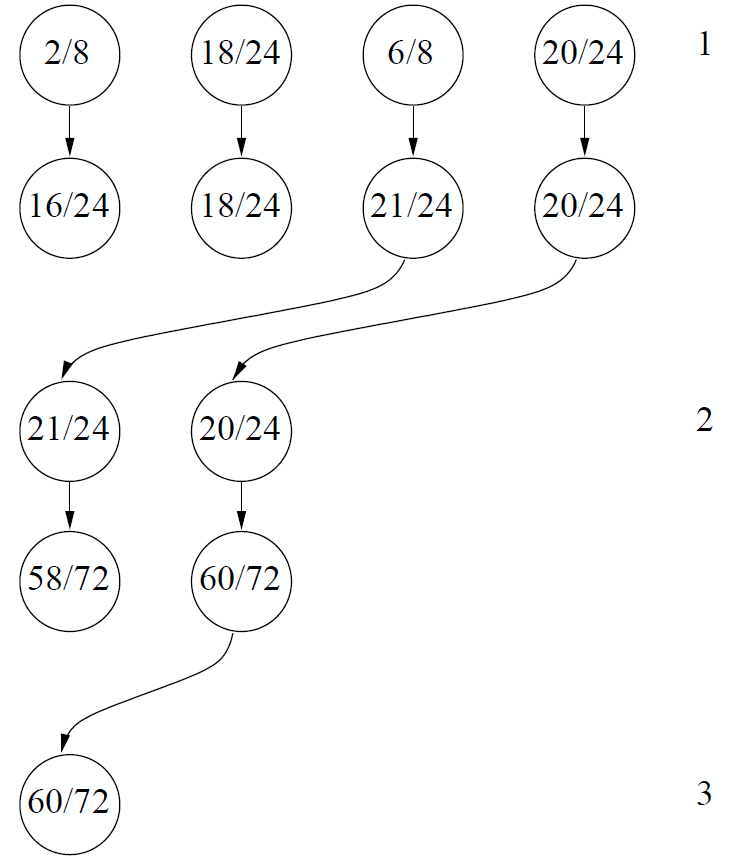
\includegraphics[width=.4\textwidth]{img/shot_topoffs.png}
	\caption{Division of 128 play-outs. The current node was previously visited 64 times~\protect\citebay{Cazenave14SHOT}.}
	\label{fig:shot-topoffs}
\end{figure}

SHOT was demonstrated to outperform UCT in NoGo, both on $9\times9$, and $19\times19$ boards, with win-rates between $75\%$ and $100\%$. However, based on the results in the article and Chapter \ref{chap:experiments}, these results were due to SHOT being significantly faster than UCT. When both algorithms are given the same budget of play-outs, different results are achieved.

Although in the original article SHOT is presented with the use of a transposition table instead of a tree, in Algorithm \ref{alg:shot} a version of SHOT using a tree of game states is presented.

\newpage
\IncMargin{1em}
\RestyleAlgo{boxruled}
\begin{algorithm2e}[ht]
\setstretch{1.1}
	\KwIn{node $p$, allocated budget $budget$}
	\KwOut{tuple containing the number of visits, $p1$ and $p2$ wins, budget used}
	\func{shot}(node $p$, $budget$):													\;
	\Indp
	\lIf{isLeaf($p$)}{$S\gets$ \func{expand}($p$)}					
	$t_s \gets \tuple{0,0,0,0}$															\;
	\If{isTerminal($p$)}{																	\label{shot:terminal}
		\func{update} $t_s$, with $budget$ wins and $budget$ visits						\;
		\KwRet{$t_s$}																	\;
	}
	\If{budget = 1} {																		\label{shot:playout}
		$r \gets$ \func{playout}($p$)													\;
		\func{update} $t_s$, with 1 budget used, 1 win, and 1 visits					\;
		\KwRet{$t_s$}																	\;
	}
	\If{$|S|$ = 1} {
		$n_0 \gets$ the single element in $S$											\;
		$t_s \gets $ \func{shot}($n_0$, $budget$)											\;
		\func{update} $p$ with $t_s$													\;
		\KwRet{$t_s$}																	\;	
	}
	$s \gets |S|$, $b_u, b \gets 0$, $S_0 \gets S$ 										\;
	\While{$s >$ 1 \textbf{and} $b_u < budget$} {											\label{shot:cycle}
	$b \gets b + \displaystyle\max{\left(1, \floor[\bigg]{\frac{p.budgetSpent + budget}{s\times\ceil{log_2{|S|}}}}\right)}$ \;	\label{shot:budgeting}
		\For{i=0 \emph{\KwTo} s}{															\label{shot:round}
			$n_i \gets$ node $n$ at rank $i$ of $S_k$									\;
			$b_i \gets b - n_i.visits$													\;  \label{shot:topoff}
			\If{$b_i > 0$} {
				\If{$p$ is root \textbf{and} $i = 0$ \textbf{and} $s = 2$} {
					\tcp{Spend any left-over budget on the empirically best node}
					$b_i \gets \max{(b_i, budget - b_u - (b - n_1.visits))}$				\;
				}
				$b_i \gets \min{(b_i, budget - b_u)}$										\;
				$\tuple{v, w_1, w_2, b_{u, n_i}}_i \gets$ \func{shot}($n_i$, $b_i$)			\;
				\func{update} $p, b_u,$ and $t_s$ with $\tuple{v, w_1, w_2, b_{u, n_i}}_i$	\;
			}
			break if $b_u \geq budget$													\;
		}
		$s \gets s - \floor{\nicefrac{s}{2}}$, $k \gets k + 1$									\;
		$S_{k} \gets$ $S_{k-1}$ sorted in descending order						\;
	}
	\func{update} $p.budgetSpent$ with $b_u$											\;
	\Indm
	\KwRet{$t_s$}
  \caption[Sequential Halving applied to Trees (SHOT)]{Sequential Halving applied to Trees (SHOT)~\protect\citebay{Cazenave14SHOT}. \label{alg:shot}}
\end{algorithm2e}
\DecMargin{1em}

\newpage
SHOT recursively performs Sequential Halving until either a terminal state is encountered (line \ref{shot:terminal}), or the available budget for the current node is 1 (line \ref{shot:playout}). Because multiple play-outs can be performed from a single recursive call, a tuple $t_s$ is maintained containing: 1) the budget used $b_u$, 2) the number of wins per player $w_1$ and $w_2$, and 3) the number of visits $v$. $v$ differs from $b_u$, because visiting a terminal node spends no budget, but performing a play-out does, and in both cases the visit count of the node should be increased.

A disadvantage of SHOT is that it cannot be terminated any time, and requires a-priori knowledge of the available budget. The pure exploration policies discussed in Chapter \ref{chap:mab} guarantee a low simple regret on the recommendation only after all available $T$ simulations are performed. Therefore, they cannot be terminated, or asked for a reasonable recommendation before this limit is reached.

This leads to another concern when using any pure exploration policy recursively. As discussed in Chapter \ref{chap:mab}, UCT has the advantage of converging to maximum back-propagation over time. Giving the formal guarantee that suboptimal nodes are selected at most $O(\ln{n})$ times. This ensures that over time, values accumulated at nodes approximate the best-reply to its move. With a policy such as Sequential Halving this guarantee is related to the available budget and the branching factor. In fact, the two empirically best nodes are sampled an equally, however different their reward may be. Moreover, for a node with a set of children $S$, the worst $\frac{|S|}{2}$ of these are sampled at least at total of $\floor{\frac{T}{\ceil{log_2{|S|}}}}$ times. In many games there are only a hand full of good moves given a position, and to evaluate a node we should find its best-reply. By using Sequential Halving throughout the tree, values back-propagated do not converge in the same manner as UCT, as such values of internal nodes are constituted of more overall averages over their children.

% --------------------------------------------------------------
% ------------------- ::::::: H-MCTS ::::::: -------------------
% --------------------------------------------------------------
\chapter{A Hybrid MCTS}
\label{chap:hybmcts}
\begin{chaptercontents}
The main contribution of this thesis, a hybrid version of MCTS named H-MCTS, which combines simple and cumulative regret minimizing selection policies into a single search technique.
\end{chaptercontents}
\section{Introduction}
As a selection policy for MCTS, UCT minimizes cumulative regret over time throughout the tree. At internal nodes, minimizing cumulative regret ensures an expected rewarding node is visited more often. UCT converges to a greedy selection policy, where at each iteration only the expected best node is selected. In effect, the average rewards at parents converge to the maximum over their children, \ie UCT converges to maximum back-propagation on a stable distribution~\citebay{kocsis2006bandit}. Secondly, UCT ensures that search time is divided efficiently, as selecting suboptimal nodes is limited by $O(\ln(n))$ where $n$ is the number of trials~\citebay{auer2002using,kocsis2006bandit}. However, such a selection policy offers a simple regret that decreases at best polynomially fast~\citebay{Bubeck11Pure}. These two properties are not only practical when long deliberation times are feasible, rather, it is possible to terminate UCT any time to obtain a reasonable approximation of the utility of a decision. During search this means that at each ply and at any time, MCTS can be asked for a best response to a parent's move.

In contrast, pure exploration algorithms, designed to minimize simple regret in multi-armed bandits such as Successive Rejects~\citebay{audibert2010best} and Sequential Halving~\citebay{Karnin13SH}, discussed in Chapter~\ref{chap:mab}, explore all options without specifically exploiting the best one. This results in a lower bound on simple regret only after all simulations have been performed. As such, to be used effectively, these algorithms can not be terminated at \emph{any time}, and have a lower formal guarantee on the number of suboptimal selections made. Moreover,~\citeaby{Bubeck11Pure} have shown that at moderate deliberation times, a modified UCB selection policy, which includes an exploration constant not unlike UCT, resulted in a better bound on simple regret than algorithms designed to minimize it. Relating these findings to MCTS, and assuming that, given sufficient time, minimizing simple regret gives a lower simple regret than UCT, we may choose to use a simple regret minimizing algorithm whenever sufficient trials can be performed, and switch to UCT when the computational budget is smaller.

Inspired by the analysis and discussions in Chapters \ref{chap:mab} and \ref{chap:mctssr}, a new MCTS variant is proposed named Hybrid MCTS (H-MCTS). H-MCTS initializes with an exploratory depth-limited search, applying a specific simple regret minimizing policy. After reaching a node where computational budget per node is smaller than a set limit, the algorithm switches to the UCT selection policy. 
\vspace{2 mm}

Section \ref{sec:hybmcts} gives an introduction and analysis of H-MCTS. Next, Section \ref{sec:hybmctssolver} details the implementation of MCTS-Solver~\citebay{Winands2008}, designed to solve positions within the tree, for H-MCTS. Finally, in Section \ref{sec:ulb_h-mcts}, an enhancement for SHOT and H-MCTS is introduced that reduces the number of poor nodes selected based on their upper bounds overlapping with their best sibling's lower bound.
\newpage
\section{Hybrid MCTS}
\label{sec:hybmcts}

Recall that in the MAB context, in which simple regret minimization is appropriate, only the final recommendation made by an algorithm has an effect on the agent's reward. In game play this holds for the nodes of the search tree at the first ply. Only after performing all simulations is a recommendation made which affects the state of the game being played. Nodes deeper in the tree have an implicit effect on this decision. Because the shape of an MCTS tree is directly related to the potential reward of internal nodes, promising nodes are selected more often to grow the tree in their direction. This both enforces the confidence of the reward of promising nodes, but also ensures that their reward can be falsified based on results deeper in the tree.

\begin{figure}[ht]
	\centering
	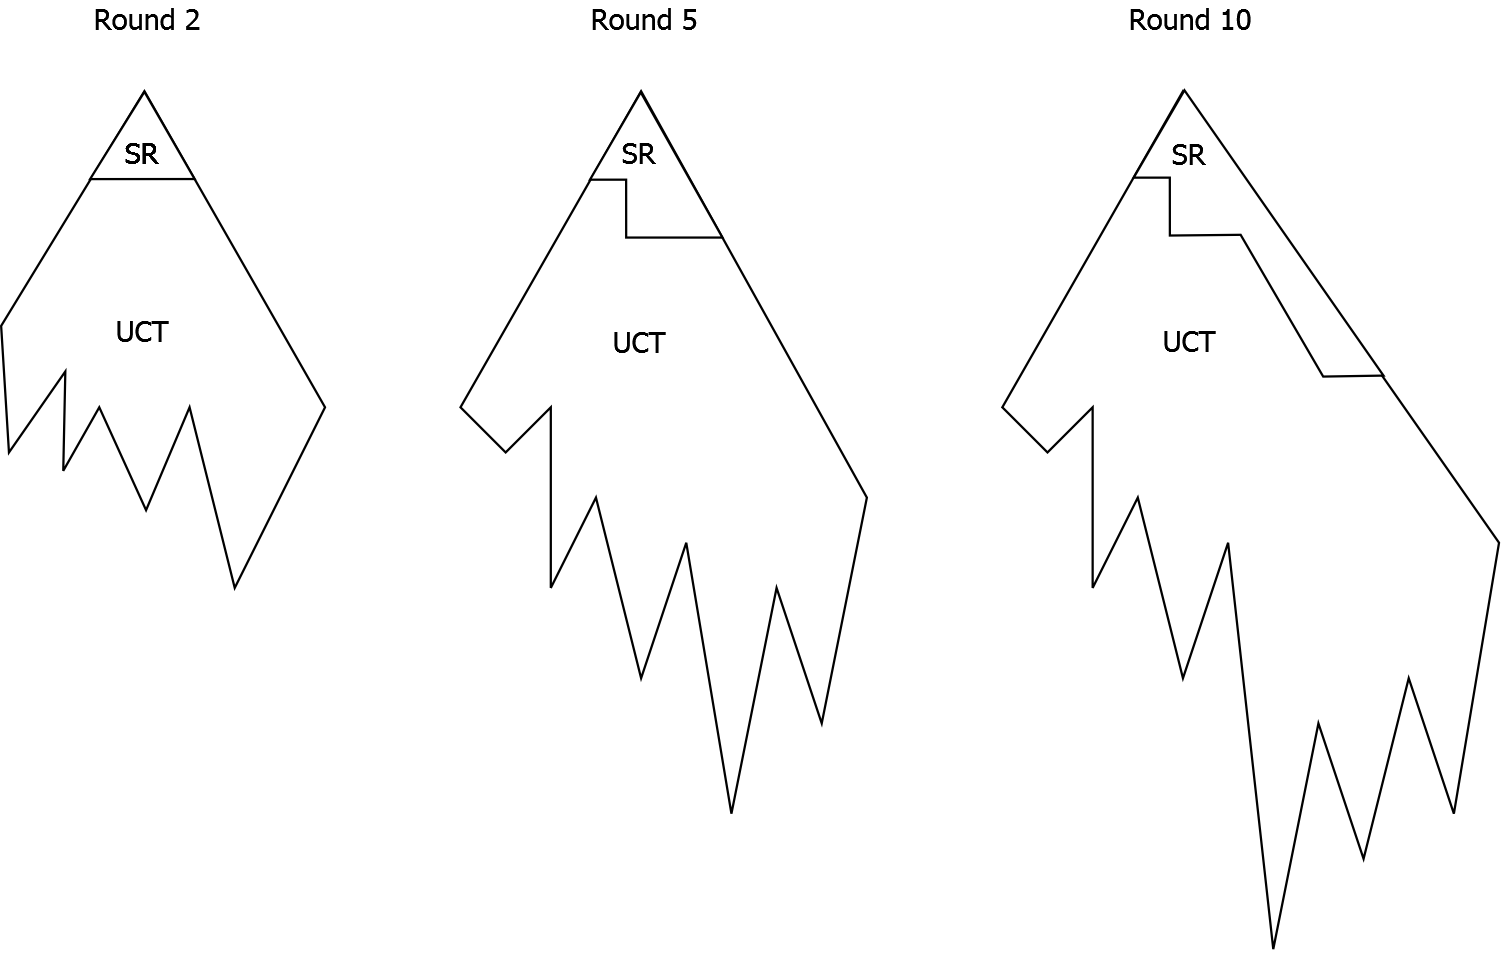
\includegraphics[width=.8\textwidth]{img/H-MCTS.png}
	\caption{Example progression of H-MCTS. In the top part of the tree (SR), simple regret is minimized, in the lower part UCT minimizes cumulative regret. The rounds represent the Sequential Halving round at the root.}
	\label{fig:h-mcts_trees}
\end{figure}

Treating a game tree as a recursive multi-armed bandit thus reveals different objectives for the distinct plies of the tree. At the root, simple regret should be as low as possible, since the recommendation of the algorithm is based on the first ply of the tree. Further down, we want to both sample efficiently, avoiding time wasted on bad options, and back-propagate correct values from leafs to their ancestors. Where the former can be achieved by using selection policies such as Successive Rejects or Sequential Halving, the latter, as discussed in Section \ref{sec:mabmcts} of Chapter \ref{chap:mab} is inherently performed by UCT. Intuitively, this leads to the belief that we should only minimize simple regret at the root, and use UCT throughout the rest of the tree, as suggested by~\citeaby{tolpin2012mcts}. 
However, considering that at any node, based on the MinMax principle, we want to find the \emph{best reply} to the action of the parent. It may also be beneficial to ensure a low simple regret on that particular move because this could intrinsically lead to an improved evaluation of the parent. Using the SHOT technique, we can apply Sequential Halving recursively, essentially combining recursive simple and cumulative minimization in a single search tree, as depicted in Figure~\ref{fig:h-mcts_trees}.

\begin{figure}[ht]
	\centering
	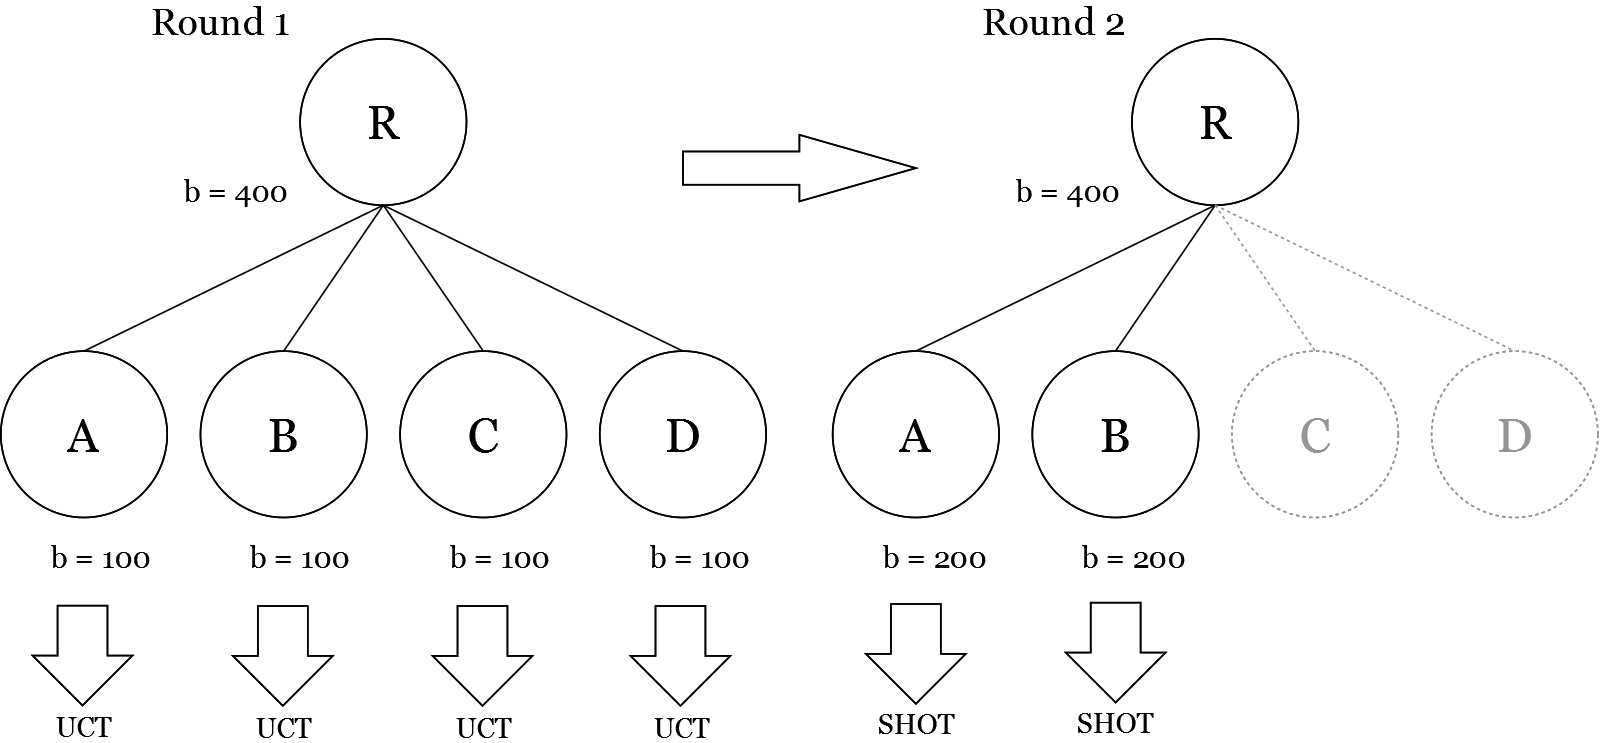
\includegraphics[width=.8\textwidth]{img/H-MCTS_Rounds.png}
	\caption{Example rounds of H-MCTS with a budget limit $B = 150$. During the first round SHOT is used only at the root R. In round 2, the budget per node is higher, and SHOT is used recursively at nodes A and B.}
	\label{fig:h-mcts_rounds}
\end{figure}

Using a selection policy based on both SHOT and UCT, Hybrid MCTS (H-MCTS) combines simple and cumulative regret minimization in a tunable algorithm. Based on the results in~\citebay{Bubeck11Pure}, which show that given a low sampling budget, UCB empirically realizes lower simple regret. The proposed technique switches from Sequential Halving to UCT whenever the computational budget is below the budget limit $B$. Consequently, the search tree is composed of a \emph{simple regret tree} at the root, and \emph{UCT trees} rooted at the leafs of the simple regret tree. As shown in Figure~\ref{fig:h-mcts_trees}, initially the simple regret tree is shallow because the computational budget per node is small. Later, when the budget per node increases due to nodes being removed from selection as per Sequential Halving, the simple regret tree grows deeper. Note that, since the root's children are sorted in descending order, the left part of the simple regret and UCT trees are always the deepest, since its root is selected the most (Figure~\ref{fig:h-mcts_rounds}).
\newpage
\IncMargin{1em}
\begin{algorithm2e}
\setstretch{1.1}
	\KwIn{node $p$, allocated budget $budget$}
	\KwOut{$t_s$: number of play-outs, $p1$ and $p2$ wins}
	\vspace{0.1cm}
	\func{h-mcts}(node $p$, $budget$):												\;
	\Indp
	\lIf{isLeaf($p$)}{$S\gets$ \func{expand}($p$)}					
	$t_s \gets \tuple{0,0,0}$														\;		
	\If{isTerminal($p$)}{															\label{h-mcts:terminal}
		\func{update} $t_s$, with $budget$ wins and visits							\;
		 \KwRet{$t_s$}
	}
	$b \gets \max{\left(1, \floor[\bigg]{\frac{p.budgetSpent + budget}{s\times\ceil{log_2{|S|}}}}\right)}$ \; \label{h-mcts:budgetlimit}
	\If{not isRoot($p$) \textbf{and} $b < B $}{
		\For{i=0 \emph{\KwTo} budget}{
			$\tuple{v, w_1, w_2}_i \gets$ \func{uct}($p$)							\;
			\func{update} $p, t_s$ with $\tuple{v, w_1,w_2}_i$						\;
		}
		\KwRet{$t_s$}
	}
	$b_u, k \gets 0$\; $S_0 \gets S$\; $s \gets |S|$								\;
	\Repeat{$b_u \geq budget$ \textbf{or} $s < 2$} {								\label{h-mcts:shot}
		\For{i=0 \emph{\KwTo} s}{
			$n_i \gets$ node $n$ at rank $i$ of $S_k$								\;			
			\If{$b > n_i.visits$} {
				$b_i \gets b - n_i.visits$											\;
				\lIf{$i = 0$ \textbf{and} $s = 2$} { $b_i \gets \max{(b_i, budget - b_u - (b - n_1.visits))}$ }
				$b_i \gets \min{(b_i, budget - b_u)}$								\;
				$\tuple{v, w_1, w_2}_i \gets$ \func{h-mcts}($n_i$, $b_i$)			\;
				\func{update} $p, b_u$, and $t_s$ with $\tuple{v, w_1, w_2}_i$		\;	\label{h-mcts:update}
			}
			break if $b_u \geq budget$												\;
		}
		$s \gets s - \floor{\nicefrac{s}{2}}$, $k \gets k + 1$							\;
		$S_{k} \gets$ $S_{k-1}$, with the first $s$ elements sorted in descending order	\;	\label{h-mcts:sort}
		$b \gets b + \max{\left(1, \floor[\bigg]{\frac{p.budgetSpent + budget}{s\times\ceil{log_2{|S|}}}}\right)}$\;
	}
	\func{update} $p.budgetSpent$ with $b_u$										\;
	\Indm
	\KwRet{$t_s$}
  \caption{Hybrid Monte-Carlo Tree Search (H-MCTS). \label{alg:h-mcts}}
\end{algorithm2e}
\DecMargin{1em}

H-MCTS is outlined in Algorithm~\ref{alg:h-mcts}. Similar to UCT and SHOT, on line~\ref{h-mcts:terminal} terminal conditions are handled. Followed by the main feature of the algorithm on line~\ref{h-mcts:budgetlimit} where the initial simulation budget $b$ for each child of the current node is computed. Based on $b$, a decision is made whether to progress into the UCT tree if $b<B$ or, if $b \geq B$ to continue with SHOT. Note that, the $b<B$ check is overridden at the root, since only one cycle is initiated there. Assuming the allocated budget is large, at the root simple regret minimization is preferred over cumulative regret minimization. From line~\ref{h-mcts:shot} the algorithm is similar to the Sequential Halving portion of SHOT. As in SHOT, because multiple play-outs are back-propagated in a single descent from root to leaf, the algorithm returns a tuple $t_s$, which contains: 1) the number of visits $v$, and 2) the number of wins per player $w_1$ and $w_2$. On line~\ref{h-mcts:update}, the budget used $b_u$ is incremented by $v$ from the results returned by the recursion. Moreover, the current node's statistics are updated, alongside the cumulative tuple $t_s$, which are returned to the node's parent. UCT also maintains a tuple of statistics such that it can return the same $t_s$ to the simple regret tree. For the UCT tree, any implementation can be used, as long as it is adapted to return $t_s$ and update the $budgetSpent$ value alongside the usual node's visit count. Because any UCT node in the tree can be ``converted'' to a simple regret node at any time, when $b>B$ on line~\ref{h-mcts:budgetlimit}. 

As with MCTS, H-MCTS can be separated in four discrete steps:
\begin{enumerate}
\item \textbf{Budgeting}: A budget is determined for each child. Based on the budget, we enter the UCT tree, or remain in the simple regret tree. If we enter the UCT tree, the four basic MCTS steps apply.
\item \textbf{Selection}: In the simple regret tree, nodes are sampled based on Sequential Halving. Nodes in the simple regret tree are assigned a budget, to be spent in their rooted UCT tree, in which play-outs are initiated.
\item \textbf{Removal}: Based on the results obtained, children are removed from selection. A new Sequential Halving round starts with half of the best children from the previous round. If the budget is spent, the currently accumulated results are back-propagated.
\item \textbf{Back-propagation}: Since H-MCTS is performed depth-first, the final result is only available after all budget is spent. This results in simultaneous back-propagation of numerous results in the simple regret tree.
\end{enumerate}

H-MCTS shares its disadvantage of not being able to return a recommendation at any time with SHOT. It must know its exact computational budget beforehand. However, it does make use of the fact that UCT is any time. Suppose a node was selected and expanded by H-MCTS, then at each time in the simple regret tree, nodes have an appropriate value based on the results back-propagated by UCT. Thus, when SHOT finishes a round by sorting the nodes by their accumulated values on line~\ref{h-mcts:sort}, UCT's any time property ensures nodes have a representative value.

When all $T$ simulations have been performed, H-MCTS recommends the single remaining node $n_0 \in S$ at the root. Note that, this is not necessarily the one with the highest value, it is possible that the best node's value has decreased after several rounds. However, we cannot assume that the values of the previously removed nodes do not also decrease given more samples. Therefore, because most samples were spent on $n_0$, we are the most confident in its value. Other nodes with less visits may have higher values, but the confidence in these values is much lower. A possible solution to this problem presents itself in the manner that $S_k$ is constructed, on line~\ref{h-mcts:sort}. An alternative would be to setup each round's subset of nodes as follows: $S_k \gets S$ sorted in descending order. This way, nodes that were previously removed from selection can `return', and replace nodes whose value decreased.

To a lesser extent, H-MCTS also shares the speed benefit of SHOT. However, because a large part of the search tree is composed of the UCT tree, based on the budget limit $B$ H-MCTS still spends more time in the tree than SHOT overall. However, given a lower budget limit $B$, H-MCTS can be made to run faster by increasing the ratio of the simple regret tree related to the UCT tree.

\subsection{Budgeting}
In the scheme presented, a limit on the available budget determines whether to continue in the simple regret tree. However, other methods, such as a fixed depth limit for the simple regret tree, or a time-partitioned method, can be viable. Though, based on the simple regret theory, pure exploration methods only provide empirically better simple regret than UCT, given a sufficiently large budget. Given a low budget, UCT with a properly tuned constant should be preferred~\citebay{Bubeck11Pure}.

The budget limit $B$ is compared to SHOT's budget allocation:
\begin{equation}
	b = \floor[\bigg]{\frac{p.budgetSpent + budget}{s\times\ceil{log_2{|S|}}}},
\end{equation}
which includes the budget previously spent at the node.

Whenever a Sequential Halving round can be initiated with a budget per child higher than $B$, we continue in the simple regret tree. Otherwise the budget is assigned to UCT, which runs $b$ simulations, and returns the result of their play-outs. Play-outs are only ever initiated in the UCT tree, since UCT immediately takes advantage of the values stored at nodes. Whereas Sequential Halving selects all children $b$ times in the first round regardless of their prospects. 

\subsection{Selection}
Selection is performed by uniformly distributing the assigned budget according to the method used in SHOT. However, in H-MCTS any left-over budget is spent in the final round of Sequential Halving, as opposed to spending all residual budget at the root's best child. This ensures that internal nodes' best-replies are selected more often, improving the confidence in their valuation, and of their parents value.

Note that, although Sequential Halving is presented as the simple regret algorithm in H-MCTS, it is certainly possible to replace it with a different selection policy, such as Successive Rejects, or another form of sequential reduction of nodes.

\subsection{Removal}
Since it is possible to visit a node more than once with a new budget, children are merely ``excluded'', instead of removed, from selection. The current list of selection candidates $S_k$ consists of all children sorted from 0 to $s$. Whenever a new budget is assigned to a node, all the previously excluded children are returned so $S_0$, and a new Sequential Halving cycle can begin.

\subsection{Back-propagation}

Typically in MCTS, results of all play-outs are back-propagated and accumulated at every ancestor of the expanded leaf, \ie \emph{average back-propagation}. To determine a node's value, its descendants should be selected such that the (expected) best ones are sampled most often. In the classic MiniMax case, a node's value is determined by the value of its best-reply. In MCTS, this idea is not explicit, over time a node's value converges to the value of its best-reply. However, when a node is insufficiently sampled, the best we can do is to assign it the current average value of its children.

Whereas UCT selects only promising nodes when it can, Sequential Halving samples all nodes in the current subset, each round. This means that the statistics collected at the parent of a given node do not reflect the best-reply to its move. Moreover, unlike Sequential Halving, UCT can be asked for a recommendation at any time, this means that a node explored by UCT has a representative value at any time. With Sequential Halving, intermediate averages of a node explored by the selection policy may be under-evaluated. Recall that the best and second best children are sampled equally often, in case there exists only a single best-reply to a parent's move, this means that its value never reflects that of its best-reply. This is depicted in an example in Figure~\ref{fig:seq_halv_bp}, where the parent is under-evaluated as it is an expected win for the player to move, whereas the parent's value represents a predicted loss. When this node is reselected with new budget to allocate, this situation does not improve, because Sequential Halving samples all nodes, not just the best one.

\begin{figure}[h]
	\centering
	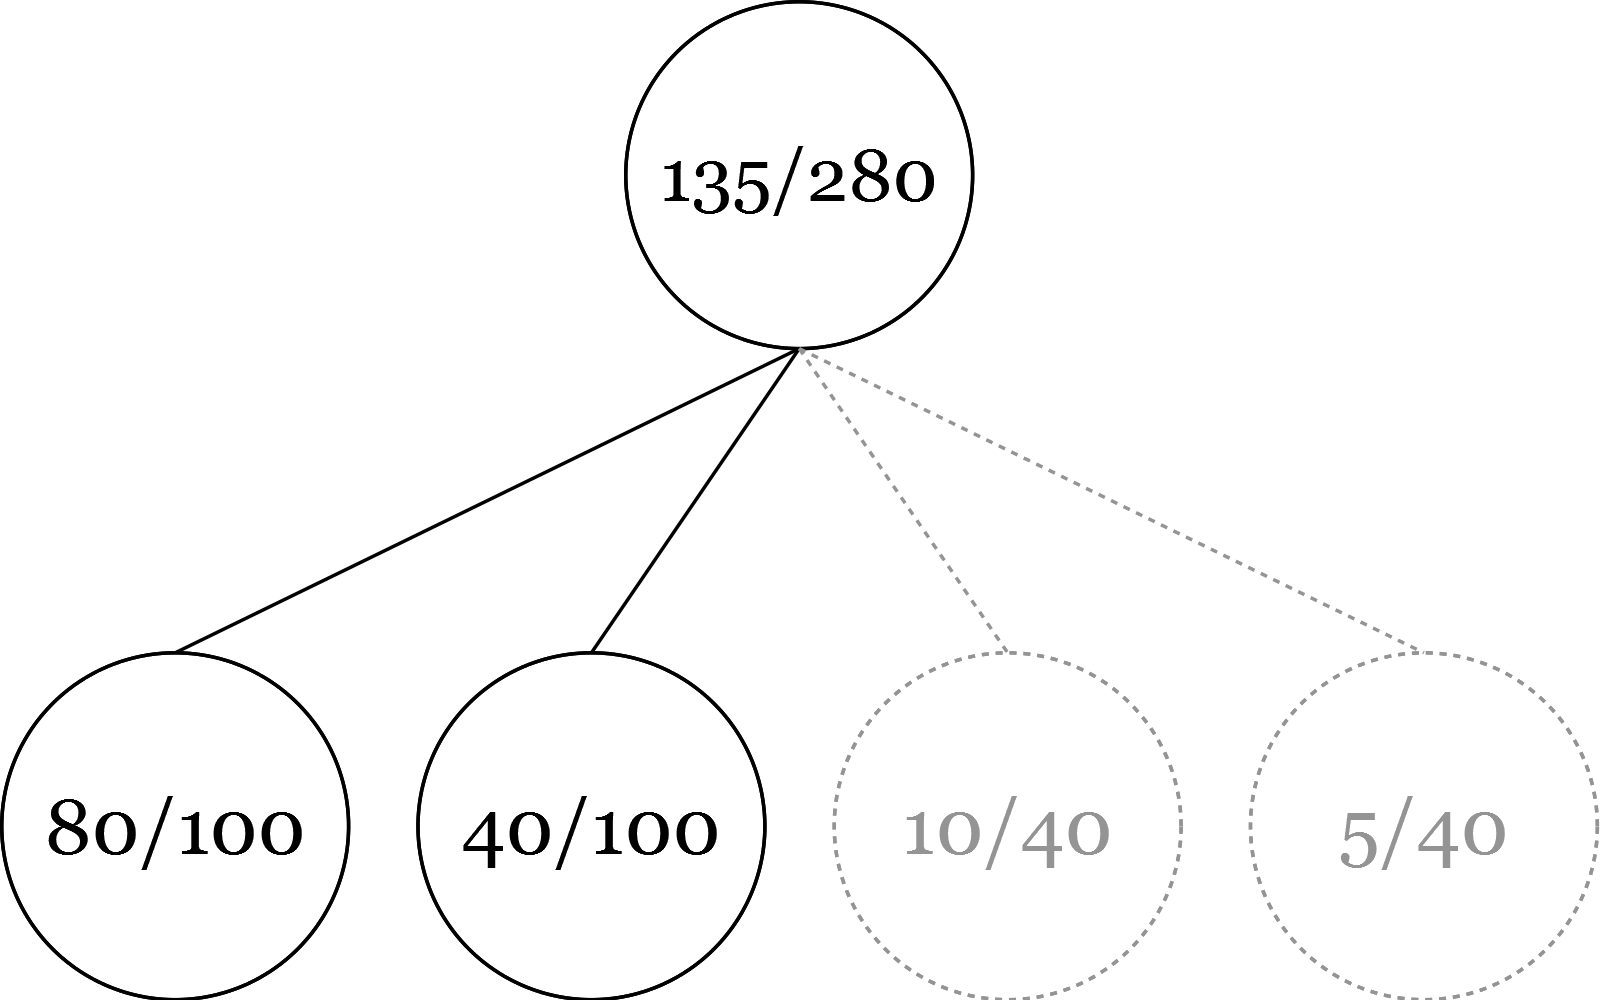
\includegraphics[width=.55\textwidth]{img/seq_halv_bp.png}
	\caption{Average back-propagation and Sequential Halving example. The parent's value $0.48$, whereas the value of the best-reply is $0.8$.}
	\label{fig:seq_halv_bp}
\end{figure}

As an alternative to average back-propagation in the simple regret tree, \emph{maximum back-propagation} sets the value of each node to the maximum over their descendants. However, because nodes explored by Sequential Halving can only provide a recommendation at time $T$, the best node's intermediate values may be incorrect. Moreover, considering that the number of visits per ply declines proportional to the branching factor, deeper nodes that are sampled infrequently may only appear to have a good value due to insufficient sampling. Back-propagating such a node's value overrules many samples performed in the rest of the tree, disregarding many of the samples taken in potentially large sub-trees with higher confidence in their value.

The problem of back-propagation remains open. According to the theory, full exploration selection policies cannot give a recommendation at any time. However, in a tree, node's values should have a representative value at any time for bot UCT and Sequential Halving to be able to select promising nodes, or sort nodes by value, respectively. In Section~\ref{sec:ulb_h-mcts}, an enhancement to Sequential Halving is discussed, which potentially reduces the number of suboptimal nodes sampled. As such, we can ensure that Sequential Halving converges to a best-reply over time.

\newpage
\section{Hybrid MCTS-Solver}
\label{sec:hybmctssolver}

In the form presented in Algorithm~\ref{alg:h-mcts}, H-MCTS cannot solve proven wins or losses in the simple regret tree. Although we can employ the MCTS-Solver proposed by~\citeaby{Winands2008} in the UCT tree, the technique requires adaptation to Sequential Halving to be able to solve nodes in the simple regret tree. The main issue here is that when a solved child is encountered, the current round is interrupted to determine whether the node itself is solved as well. This leads to three different possible cases, in which this interruption can be encountered, and properly handled. Note that it is assumed that values are according to negamax, such that at each node, children's rewards are stored with respect to the player to move.
\begin{enumerate}
\item A solved win is encountered, in this case, we immediately want to remember this node and back-propagate to the parent. Any residual budget remains unspent in the current round.
\item A solved loss is encountered, but not all siblings lead to a loss. According to~\citeaby{Winands2008} it is appropriate in this case to count the visit as a loss. However, since there still exist nodes that do not lead to a loss, we have to ensure the solved node is not reselected. If it is reselected, a potentially high budget may be spent on the node, which results in an under evaluation of the parent.
\item A solved loss is encountered, and all siblings lead lead to a loss. In this case the parent is a win and we should back-propagate immediately. Any residual budget remains unspent in the current round.
\end{enumerate}
\begin{figure}[hb]
	\centering
	\includegraphics[width=.6\textwidth]{img/solver.png}
	\caption{H-MCTS Solver removing a proven loss from selection. In the second round, node B is determined to be a proven loss, node C is returned to selection to fill the opened position.}
	\label{fig:h-mcts_solver}
\end{figure}

When running Sequential Halving, the first and last cases can be handled similar to the MCTS-Solver. The second case potentially leaves the assigned budget partially unspent. Because some children have been identified as a loss, while other unsolved options still remain, the proven losses should be removed from selection. Moreover, any budget left unspent due to this should be ``brought over'' to the next round, which starts with a reduced set of nodes. When a proven loss is discarded from selection, all children following this node move one position left, possibly returning an unsolved node to the current selection, as depicted in Figure~\ref{fig:h-mcts_solver}. If there is no unsolved node to return, the set of remaining arms is reduced only if it is smaller than $s - \floor{\nicefrac{s}{2}}$, \ie the current subset size in the next round. 

\IncMargin{1em}
\begin{algorithm2e}
\setstretch{1.0}
	\KwIn{node $p$, allocated budget $budget$}
	\KwOut{$t_s$: number of play-outs, $p1$ and $p2$ wins, solved player}
	\vspace{0.1cm}
	\func{h-mcts-solver}(node $p$, $budget$):										\;
	\Indp
	\lIf{isLeaf($p$)}{$I, S\gets$ \func{expand}($p$)}								\label{hs:children}
	$t_s \gets \tuple{0,0,0,0}$														\;		
	$b \gets \max{\left(1, \floor[\bigg]{\frac{p.budgetSpent + budget}{s\times\ceil{log_2{|S|}}}}\right)}$ \; 
	\If{$p$ is not root \textbf{and} $b < B $}{
		\For{i=0 \emph{\KwTo} budget}{
			$\tuple{v, w_1, w_2, s}_i \gets$ \func{uct-solver}($p$)						\;
			\func{update} $p, t_s$ with $\tuple{v, w_1,w_2, s}_i$							\;
		}
		\KwRet{$t_s$}
	}
	$b_u, k \gets 0$, $S_0 \gets S$, $s \gets |S_0|$\;
	\Repeat{$b_u \geq budget$} {														\label{hs:shot}
		$b_r \gets 0$																\; \label{hs:resid}
		\For{i=0 \emph{\KwTo} $s$}{
			$n_i \gets$ node $n$ at rank $i$ of $S_k$								\;
			\If{$n_i$ is not solved} {			
				\If{$b > n_i.visits$} {
					$b_i \gets b - n_i.visits$											\;
					\lIf{$i = 0$ \textbf{and} $s = 2$} { $b_i \gets \max{(b_i, budget - b_u - (b - n_1.visits))}$ }
					$b_i \gets \min{(b_i, budget - b_u)}$								\;
					$\tuple{v, w_1, w_2, s}_i \gets$ \func{h-mcts-solver}($n_i$, $b_i$)	\;
					\func{update} $p, b_u$, and $t_s$ with $\tuple{v, w_1, w_2, s}_i$		\;
				}
			}
			\uIf{$n_i$ is a win \textbf{or} $(n_i$ is a loss \textbf{and} $\forall n \in S: (n$ is a loss$))$}{
				set the solved player in $t_s$									\; \label{hs:solved}
				\func{update} $p.budgetSpent$ with $b_u$						\;
				\KwRet{$t_s$}													\;
			} \ElseIf{$(n_i$ is a loss \textbf{and} $\exists n \in S: (n$ is not a loss$))$}{
				$b_r \gets b_i - v$												\; \label{hs:update_resid}				
			}
			break if $b_u \geq budget$											\;
		}
		remove all solved nodes from $S$ and $S_k$								\;  \label{hs:remove}
		$s \gets s - \floor{\nicefrac{s}{2}}$, $k \gets k + 1$						\;
		$s \gets \min{(s, |S|)}$												\; \label{hs:size_min}	
		$S_{k} \gets$ $S_{k-1}$, with the first $\max{(2, s)}$ elements sorted in descending order	\;						\; \label{hs:sort}	
		\lIf{$s = 1$} {$b \gets b + (budget - b_u)$}
		\Else {	
			$b \gets b + \max{\left(1, \floor[\bigg]{\frac{p.budgetSpent + budget}{s\times\ceil{log_2{|S|}}}}\right)}$ \;
			$b \gets b + \ceil{\nicefrac{b_r}{s}}$														\; \label{hs:incr_budget_resid}
		}
	}
	\func{update} $p.budgetSpent$ with $b_u$										\;
	\Indm
	\KwRet{$t_s$}
  \caption{Hybrid Monte-Carlo Tree Search Solver (H-MCTS-Solver). \label{alg:h-mcts-solver}}
\end{algorithm2e}
\DecMargin{1em}
\newpage
H-MCTS Solver is outlined in Algorithm~\ref{alg:h-mcts-solver}. The general procedure when a solved node is encountered is straightforward in the case of a solved win, and when all children are solved losses. The $budgetSpent$ is updated and the function immediately returns. The tuple $t_s$ now also contains a `solved' field, which holds the index of the player for which the node is solved. In this case the \func{update} function updates the node accordingly by setting the $isSolved$ flag. When an isolated proven loss is encountered, \ie not all siblings are losses, then we should not sample that node again, since it would under-evaluate the parent. This possibly leaves a residual budget $b_r$ declared on line~\ref{hs:resid}, which is maintained per round. When an isolated proven loss is found, the residual budget is updated on line~\ref{hs:update_resid} such that it can be spent in the next round with a reduced set of nodes, on line~\ref{hs:incr_budget_resid}. Moreover, since the isolated losses are removed from $S$ on line~\ref{hs:remove}, it is possible that $s > |S|$, which is restored on line~\ref{hs:size_min} after halving $s$. This ensures that previously removed nodes that were not proven losses can be returned to selection in case more than half of the nodes were solved in this round. On line~\ref{hs:sort} the set of children from the previous round $S_{k-1}$ is sorted, as such $|S_k| = |S|$ for each round. Therefore, when a solved loss is removed from selection, another child can take its place. Note also that on line~\ref{hs:children}, a second set $I$ contains all children. Because it is possible to remove all nodes from $S$ in case of a proven loss, $I$ is never altered and can be used to give a recommendation at the root.

Some changes are made in H-MCTS-Solver with respect to SHOT. The cycle at line~\ref{hs:shot} repeats until no more budget remains instead of repeating until a single child remains. Because it is possible that not all allocated budget is spent during a cycle, ``residual'' rounds may be required, in which the single best child is the only one remaining. Sampling this child more frequently is never problematic, because at each node we are most interested in sampling the best-reply when identified.

\newpage
\section{Upper and Lower Bounds for H-MCTS}
\label{sec:ulb_h-mcts}
A disadvantage of Sequential Halving applied to game trees is that nodes that can never improve on the current best-reply are sampled relatively frequent. Although this is theoretically sound in providing lower guarantees on simple regret, practically it means that nodes are often sampled when it is clearly futile to do so. 

For example, consider a set of 5 nodes $S_1$, in which there exists one node with a true mean $\mu^*$ of $0.7$, all other nodes have means of $-0.5$. Only a few samples are required to find out which node is the best reply. However, as shown in the example in Figure~\ref{fig:seq-halving}, the second-best node are sampled as often as the best one, and in effect the parent's value is underestimated. 

To counter this problem we can compare a child's upper confidence bound to its best sibling's lower confidence bound. In this optimistic scheme it is assumed that a node can still improve its value such that it becomes better than the current best-reply, if their respective upper and lower confidence bounds overlap. Recall from Chapter~\ref{chap:mab}, that the upper confidence bound represents the highest value a node can achieve with overwhelming probability. This approach can be inversed to acquire the lowest possible value a node can achieve,
\begin{equation}
  	n_i.value - C \times \displaystyle\sqrt{\frac{\ln{p.visits}}{n_i.visits}}.
\end{equation}
Because a sorted list of children is maintained in the simple regret tree, the best child's bound can be compared to it siblings' bounds at any time. Therefore, when selecting a node to be investigated, only if the current node's upper confidence bound overlaps with the currently estimated best-reply's lower confidence bound, should we assume that it is still possible for this node to improve upon the current best node's score. As such we can skip any node with a non-overlapping bound with the best node. This potentially saves a substantial budget which would otherwise have been spent sampling suboptimal nodes. An example of this enhancement is depicted in Figure \ref{fig:ublb}. In this example, the current best node's lower bound overlaps only with the upper bounds of nodes $B$ and $C$.

\begin{figure}[ht]
	\centering
	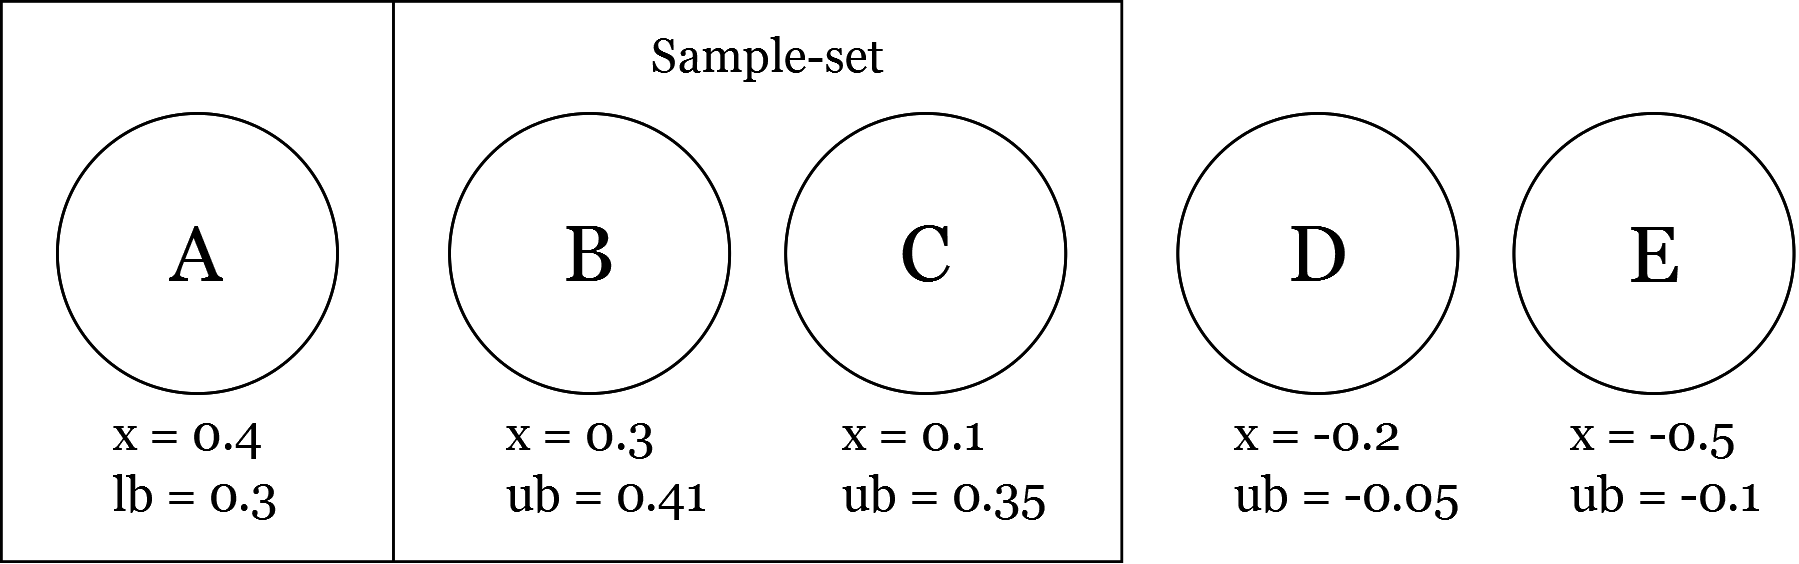
\includegraphics[width=.7\textwidth]{img/ublb.png}
	\caption{Example upper/lower bound Sequential Halving. Node A is the current empirical best, with a lower confidence bound of $0.1$. Only nodes B and C have upper confidence bounds that overlap with this lower bound. D and E are not sampled this round.}
	\label{fig:ublb}
\end{figure}

This enhancement also ensures that, over time Sequential Halving samples greedily. Given infinite samples, the lower and upper confidence bounds of two nodes should only ever overlap if they have the same value. Since, in this case only the nodes with the highest average are sampled, Sequential Halving with the Upper/Lower Bounds enhancement tends to sample only the best node(s) over time.

\IncMargin{1em}
\begin{algorithm2e}
\setstretch{0.9}
	\KwIn{node $p$, allocated budget $budget$}
	\KwOut{$t_s$: number of play-outs, $p1$ and $p2$ wins, solved player}
	\vspace{0.1cm}
	\func{h-mcts-solver}(node $p$, $budget$):										\;
	\Indp
	\lIf{isLeaf($p$)}{$I, S\gets$ \func{expand}($p$)}					
	$t_s \gets \tuple{0,0,0,0}$														\;		
	$b \gets \max{\left(1, \floor[\bigg]{\frac{p.budgetSpent + budget}{s\times\ceil{log_2{|S|}}}}\right)}$ \; 
	\If{$p$ is not root \textbf{and} $b < B $}{
		\For{i=0 \emph{\KwTo} budget}{
			$\tuple{v, w_1, w_2, s}_i \gets$ \func{uct-solver}($p$)						\;
			\func{update} $p, t_s$ with $\tuple{v, w_1,w_2, s}_i$							\;
		}
		\KwRet{$t_s$}
	}
	$b_u, k \gets 0$, $S_0 \gets S$, $s \gets |S_0|$\;
	\Repeat{$b_u \geq budget$} {
		$b_r \gets 0$																\;
		\For{i=0 \emph{\KwTo} $\min{(s,|S_k|)}$}{
			$n_i \gets$ node $n$ at rank $i$ of $S_k$								\;
			\If{$n_i$ is not solved} {			
				\If{$b > n_i.visits$} {
					$b_i \gets b - n_i.visits$											\;
					\lIf{$i = 0$ \textbf{and} $s = 2$} { $b_i \gets \max{(b_i, budget - b_u - (b - n_1.visits))}$ }
					$b_i \gets \min{(b_i, budget - b_u)}$								\;
					\If {$i > 0$ \textbf{and} $n_i.value + C \times \sqrt{\frac{\ln{p.visits}}{n_i.visits}} < l_b$} { \label{ublb:upper_bound}
						$b_r \gets b_r + b_i$ \;									
						\textbf{continue}	\;	\label{ublb:skip}
					}
					$\tuple{v, w_1, w_2, s}_i \gets$ \func{h-mcts-solver}($n_i$, $b_i$)	\;
					\func{update} $p, b_u$, and $t_s$ with $\tuple{v, w_1, w_2, s}_i$		\;
					\lIf{$i = 0$} {$l_b \gets n_i.value - C \times \sqrt{\frac{\ln{p.visits}}{n_i.visits}}$} \label{ublb:lower_bound}
				}
			}
			\uIf{$n_i$ is a win \textbf{or} $(n_i$ is a loss \textbf{and} $\forall n \in S: (n$ is a loss$))$}{
				set the solved player in $t_s$									\;
				\func{update} $p.budgetSpent$ with $b_u$						\;
				\KwRet{$t_s$}													\;
			} \ElseIf{$(n_i$ is a loss \textbf{and} $\exists n \in S: (n$ is not a loss$))$}{				
				$b_r \gets b_i - v$												\;				
			}
			break if $b_u \geq budget$											\;
		}
		remove all solved nodes from $S$ and $S_k$								\;
		$s \gets s - \floor{\nicefrac{s}{2}}$, $k \gets k + 1$					\;
		$s \gets \min{(s, |S|)}$												\;
		$S_{k} \gets$ $S_{k-1}$, with the first $\max{(2, s)}$ elements sorted in descending order					\;	
		\lIf{$s = 1$} {$b \gets b + (budget - b_u)$}
		\Else{
			$b \gets b + \max{\left(1, \floor[\bigg]{\frac{p.budgetSpent + budget}{s\times\ceil{log_2{|S|}}}}\right)}$ \;
			$b \gets b + \ceil{\nicefrac{b_r}{s}}$\;	\label{ublb:reallo}
		}
	}
	\func{update} $p.budgetSpent$ with $b_u$										\;
	\Indm
	\KwRet{$t_s$}
  \caption{Hybrid Monte-Carlo Tree Search Solver with Overlapping Bounds. \label{alg:h-mcts-ublb}}
\end{algorithm2e}
\DecMargin{1em}

The Overlapping Bounds enhancement for H-MCTS is detailed in Algorithm~\ref{alg:h-mcts-ublb}, in which it is combined with the solver discussed in the previous subsection. On line~\ref{ublb:lower_bound} the lower confidence bound of the current best node is determined. Note that this is performed in each round, right after the best node of the round is sampled. This ensures that we have the best estimate for the current lower bound. All other children's upper confidence bounds are then compared to the current best lower bound on line~\ref{ublb:upper_bound}. If the bounds do not overlap, the node is skipped, line~\ref{ublb:skip}. Similar to the solver, the unspent budget is reserved in $b_r$, it is reallocated on line~\ref{ublb:reallo} to be spent in the next round.

% -------------------------------------------------------------------------------
% ------------------- ::::::: Experiments and Results ::::::: -------------------
% -------------------------------------------------------------------------------
\chapter{Experiments and Results}
\label{chap:experiments}
\begin{chaptercontents}
H-MCTS is thoroughly evaluated in six distinct two-player games: Amazons, AtariGo, Ataxx, Breakthrough, NoGo, and Pentalath.
\end{chaptercontents}

\section{Experimental Setup}
\label{sec:ex_setup}
In this chapter the results of the experiments performed on six two-player games are presented. H-MCTS and the games were implemented in two different engines. Amazons, Breakthrough, NoGo and Pentalath are implemented in a Java based engine. Ataxx and AtariGo are implemented in a \emph{C++} based engine.
\begin{itemize}
\item \emph{Amazons} is played on a 10$\times$10 chessboard. Players each have four Amazons that move as queens in chess. Moves consist of two parts, movement, and shooting an arrow to block a square on the board. The last player to move wins the game.
\item \emph{AtariGo}, or first-capture Go, is a variant of Go where the first player to capture any stones wins. The experiments are performed on a 9$\times$9 board.
\item \emph{Ataxx} is a game similar to Reversi. Played on a square board, players start with two stones each placed in an opposite corner. Captures are performed by moving a stone alongside an opponent's on the board. In the variant used in this paper, jumps are not allowed. The game ends when all squares are filled, or when a player has no remaining stones. The player with the most stones wins.  The experiments are performed on a 7$\times$7 board.
\item \emph{Breakthrough} is played on an 8$\times$8 board. Players start with 16 pawns. The goal is to move one of them to the opponent's side.
\item \emph{NoGo} is a combinatorial game based on Go. Captures are forbidden and the first player unable to play due to this rule, loses. The experiments are performed on a 9$\times$9 board.
\item \emph{Pentalath} is a connection game played on a hexagonal board. The goal is to place 5 pieces in a row. Pieces can be captured by fully surrounding an opponent's set of pieces.
\end{itemize}

All games use a uniform random selection policy during the play-outs, unless otherwise stated. The $C$ constant, used by UCT (Equation \ref{eq:uct}) was optimized for each game and was not re-optimized for H-MCTS, unless otherwise stated both UCT and H-MCTS use the same $C$ constant.

Because H-MCTS cannot be terminated any time we present only results for a fixed number of simulations. In each experiment, both players are allocated a budget of both 10,000 and 25,000 play-outs.
\newpage
\section{Results}
\label{sec:results}
For the tables and graphs, the results are shown with respect to the first algorithm mentioned in the captions, along with a 95\% confidence interval. For each experiment, the players' seats were swapped such that 50\% of the games are played as the first player, and 50\% as the second, to ensure no first-player or second-player bias. 

\subsection{H-MCTS and UCT}

\begin{figure}[ht]
\centering
\captionsetup{justification=centering,margin=1cm}
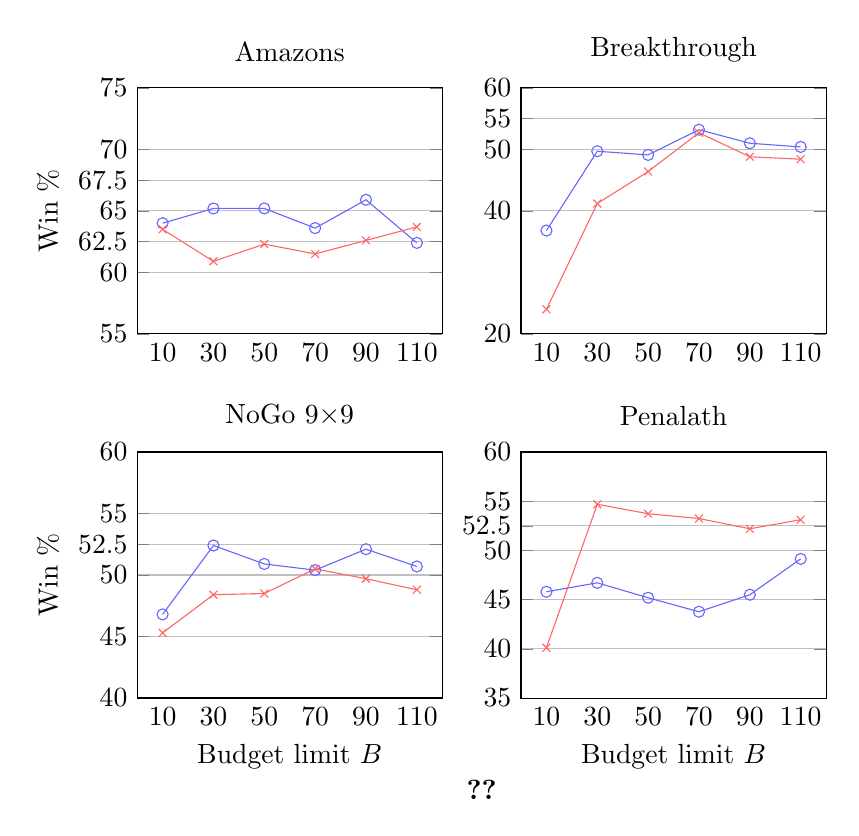
\begin{tikzpicture}
\begin{groupplot}
    [
        group style=
            {
            columns=2,
            rows=2,
            xlabels at=edge bottom,
            ylabels at=edge left,
            vertical sep= 1.5cm,
            },
        legend columns=2,
       	width  = 0.45*\textwidth,
        major x tick style = transparent,
        %ybar= 2 * \pgflinewidth,
        % bar width = 10pt,
        ymajorgrids = true,
        ylabel = {Win \%},
        xlabel= {Budget limit $B$},
        symbolic x coords={10,30,50,70,90,110},
        xtick = data,
        ytick={0,20,30,40,45,50,55,60,65,70,80},
        scaled y ticks = false,
        enlarge x limits = 0.1,
        ymin=0, ymax=80
    ]
% Amazons ----------------------------------------
\nextgroupplot[title=Amazons, ymin=55, ymax=75, ytick={55,60,62.5,65,67.5,70,75}]
\addplot[blue!60!white, mark=o, range=50:70]
	coordinates {(10, 64) +- (0,2.98) 
	(30,65.2) +- (0,2.95)
	(50,65.2) +- (0,2.95)
	(70,63.6) +- (0,2.98)
	(90,65.9) +- (0,2.94)
	(110,62.4) +- (0,3.00)};
\addplot[red!60!white, mark=x]
	coordinates {(10,63.5) +- (0,2.98)
	(30,60.9) +- (0,3.02)
	(50,62.3) +- (0,3.00)
	(70,61.5) +- (0,3.02)
	(90,62.6) +- (0,3.00)
	(110,63.7)+- (0,2.98)};
% Breakthrough -------------------------------------
\nextgroupplot[title=Breakthrough, ymin=20, ymax=60, ytick={20,40,50,55,60}]
\addplot[blue!60!white, mark=o]
	coordinates {(10, 36.8) +- (0,2.99) 
	(30,49.7) +- (0,3.1)
	(50,49.1) +- (0,3.1)
	(70,53.2) +- (0,3.1)
	(90,51) +- (0,3.1)
	(110,50.4) +- (0,3.1)};
\addplot[red!60!white, mark=x]
	coordinates {(10,24) +- (0,2.65)
	(30,41.2) +- (0,3.05)
	(50,46.4) +- (0,3.09)
	(70,52.7) +- (0,3.09)
	(90,48.8) +- (0,3.10)
	(110,48.4)+- (0,3.10)};
% NoGo --------------------------------------------
\nextgroupplot[title=NoGo 9$\times$9, ymin=40, ymax=60, ytick={20,40,45,50,52.5,55,60}]
\addplot[blue!60!white, mark=o]
	coordinates {(10, 46.8) +- (0,3.09) 
	(30,52.4) +- (0,3.1)
	(50,50.9) +- (0,3.1)
	(70,50.4) +- (0,3.1)
	(90,52.1) +- (0,3.1)
	(110,50.7) +- (0,3.1)};
\addplot[red!60!white, mark=x]
	coordinates {(10,45.3) +- (0,3.09)
	(30,48.4) +- (0,3.1)
	(50,48.5) +- (0,3.1)
	(70,50.5) +- (0,3.1)
	(90,49.7) +- (0,3.1)
	(110,48.8)+- (0,3.1)};

% Pentalath --------------------------------------------
\nextgroupplot[title=Penalath, legend to name=grouplegend, ymin=35, ymax=60, ytick={20,35,40,45,50,52.5,55,60}]
\addplot[blue!60!white, mark=o]
	coordinates {(10, 45.8) +- (0,3.11) 
	(30,46.71) +- (0,3.11)
	(50,45.19) +- (0,3.11)
	(70,43.77) +- (0,3.1)
	(90,45.5) +- (0,3.1)
	(110,49.14) +- (0,3.1)};
	\addlegendentry{10,000 play-outs}
\addplot[red!60!white, mark=x]
	coordinates {(10,40.12) +- (0,3.07)
	(30,54.69) +- (0,3.12)
	(50,53.73) +- (0,3.14)
	(70,53.24) +- (0,3.12)
	(90,52.2) +- (0,3.13)
	(110,53.12)+- (0,3.13)};
	\addlegendentry{25,000 play-outs}
\end{groupplot}

    \node (legend) at ($(group c1r2.south)!0.5!(group c2r2.south)$)
      [below, yshift=-2\pgfkeysvalueof{/pgfplots/every axis title shift}]
      {\ref{grouplegend}};

\end{tikzpicture}
     \caption[H-MCTS $B$ values]{H-MCTS vs. UCT, random play-outs. \\ Win percentages with respect to H-MCTS. 1,000 games per data point.}
     \label{fig:h-mcts_v_uct}
\end{figure}



Figure~\ref{fig:h-mcts_v_uct} gives an overview of the results for different budget limits $B$ in H-MCTS. For each game 1,000 matches were played with a budget of 10,000 and 25,000 play-outs. For Amazons, different settings of $B$ do not significantly influence the performance of H-MCTS. This is mainly due to the enormous branching factor of $\pm 4,800$ moves, at the start of the games. UCT spreads its budget out, allocating it almost randomly since it is unable to procure sufficient visits per move to decrease their confidence bounds. Unlike UCT, H-MCTS initially performs several rounds with a high number of choices, but reduces the number of nodes under consideration quickly, allowing it to focus on a subset of moves found to be promising. Mainly in Breakthrough and Pentalath does $B$ have a large impact on performance. Notably, in Pentalath we observe a significant increase in performance given a larger budget of play-outs. For NoGo, results are similar to Amazons overall, NoGo initially has 81 possible moves, and this number does not decline rapidly as the game progresses. The graphs show that the best budget limit per game does not change when the algorithm is given a higher deliberation time.

% \begin{figure}[h]
\centering
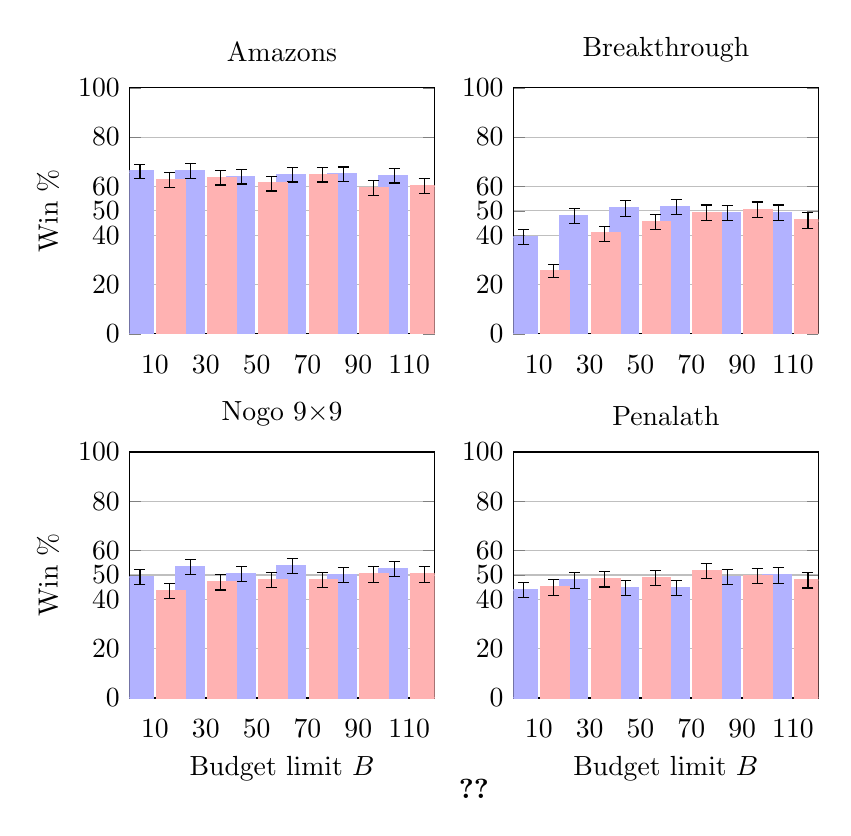
\begin{tikzpicture}
\begin{groupplot}
    [
        group style=
            {
            columns=2,
            rows=2,
            xlabels at=edge bottom,
            ylabels at=edge left,
            vertical sep= 1.5cm,
            },
       	width  = 0.45*\textwidth,
        major x tick style = transparent,
        ybar= 2 * \pgflinewidth,
        % bar width = 10pt,
        ymajorgrids = true,
        ylabel = {Win \%},
        xlabel= {Budget limit $B$},
        symbolic x coords={10,30,50,70,90,110},
        xtick = data,
        ytick={0,20,40,50, 60,80,100},
        scaled y ticks = false,
        enlarge x limits = 0.1,
        ymin=0,
        ymax=100,
    ]
% Amazons ----------------------------------------
\nextgroupplot[title=Amazons]
\addplot[blue!30!white, fill=blue!30!white, thick, error bars/.cd,
            y dir=both, error bar style={black},
            y explicit]
	coordinates {
	(10, 66) +- (0,2.94) 
	(30,66.2) +- (0,2.93)
	(50,63.9) +- (0,2.98)
	(70,64.7) +- (0,2.96)
	(90,64.9) +- (0,2.96)
	(110,64.3) +- (0,2.97)};
\addplot[red!30!white, fill=red!30!white, thick, error bars/.cd,
            y dir=both, error bar style={black},
            y explicit]
	coordinates {
	(10,62.6) +- (0,3)
	(30,63.5) +- (0,2.99)
	(50,61.1) +- (0,3.02)
	(70,64.7) +- (0,2.96)
	(90,59.3) +- (0,3.04)
	(110,60.1)+- (0,3.04)};
% Breakthrough -------------------------------------
\nextgroupplot[title=Breakthrough]
\addplot[blue!30!white, fill=blue!30!white, thick, error bars/.cd,
            y dir=both, error bar style={black},
            y explicit]
	coordinates {
	(10, 39.48) +- (0,3.03) 
	(30,47.8) +- (0,3.1)
	(50,50.95) +- (0,3.1)
	(70,51.6) +- (0,3.1)
	(90,49.2) +- (0,3.1)
	(110,49.3) +- (0,3.1)};
\addplot[red!30!white, fill=red!30!white, thick, error bars/.cd,
            y dir=both, error bar style={black},
            y explicit]
	coordinates {
	(10,25.45) +- (0,2.7)
	(30,40.78) +- (0,3.05)
	(50,45.35) +- (0,3.09)
	(70,49.3) +- (0,3.1)
	(90,50.5) +- (0,3.1)
	(110,46.1)+- (0,3.09)};
% Nogo --------------------------------------------
\nextgroupplot[title=Nogo 9$\times$9]
\addplot[blue!30!white, fill=blue!30!white, thick, error bars/.cd,
            y dir=both, error bar style={black},
            y explicit]
	coordinates {
	(10, 49.3) +- (0,3.1) 
	(30,53.3) +- (0,3.09)
	(50,50.4) +- (0,3.1)
	(70,53.6) +- (0,3.09)
	(90,50.0) +- (0,3.1)
	(110,52.5) +- (0,3.1)};
\addplot[red!30!white, fill=red!30!white, thick, error bars/.cd,
            y dir=both, error bar style={black},
            y explicit]
	coordinates {
	(10,43.6) +- (0,3.07)
	(30,47) +- (0,3.09)
	(50,48) +- (0,3.1)
	(70,48) +- (0,3.1)
	(90,50.2) +- (0,3.1)
	(110,50.2)+- (0,3.1)};

% Pentalath --------------------------------------------
\nextgroupplot[title=Penalath, legend to name=grouplegend2]
\addplot[blue!30!white, fill=blue!30!white, thick, error bars/.cd,
            y dir=both, error bar style={black},
            y explicit]
	coordinates {
	(10,44.04) +- (0,3.08) 
	(30,47.75) +- (0,3.1)
	(50,44.64) +- (0,3.08)
	(70,44.63) +- (0,3.09)
	(90,49.2) +- (0,3.1)
	(110,49.79) +- (0,3.1)};
	\addlegendentry{10,000 play-outs}
\addplot[red!30!white, fill=red!30!white, thick, error bars/.cd,
            y dir=both, error bar style={black},
            y explicit]
	coordinates {
	(10,44.96) +- (0,3.1)
	(30,48.24) +- (0,3.1)
	(50,48.75) +- (0,3.1)
	(70,51.75) +- (0,3.1)
	(90,49.6) +- (0,3.1)
	(110,47.84)+- (0,3.1)};
	\addlegendentry{25,000 play-outs}
\end{groupplot}

    \node (legend) at ($(group c1r2.south)!0.5!(group c2r2.south)$)
      [below, yshift=-2\pgfkeysvalueof{/pgfplots/every axis title shift}]
      {\ref{grouplegend2}};

\end{tikzpicture}
     \caption{H-MCTS Solver vs. MCTS-Solver with random play-outs. Win percentages with respect to H-MCTS, error bars represent 95\% c.i..}
     \label{fig:h-mcts-s_v_mcts-s}
\end{figure}



% In Figure~\ref{fig:h-mcts-s_v_mcts-s}, results are shown for different values for $B$ for H-MCTS Solver. All games were played against the MCTS-Solver. Although performance decreases overall with respect to Figure~\ref{fig:h-mcts_v_uct}, the best values determined for $B$ remain the same in both results.

\begin{table}[ht]
\centering
\tabcolsep=0.3cm
\scalebox{1.0}{
\begin{tabular}{rlll}
\hline
\multicolumn{2}{c|}{} & \multicolumn{1}{c}{\textbf{10,000}} & \multicolumn{1}{c}{\textbf{25,000}} \\ 
\textbf{Game} & \multicolumn{1}{c|}{\textbf{$B$}} & \multicolumn{1}{c}{\textbf{play-outs}} & \multicolumn{1}{c}{\textbf{play-outs}} \\ [1mm] 
\cline{1-4}
\multicolumn{2}{c|}{} \\ [-3mm]
Amazons &\multicolumn{1}{l|}{50}			    	& {\bf{65.2}} $\pm$ 3.0 		& {\bf{62.3}} $\pm$ 3.0 		\\ [.5mm] 
AtariGo 9$\times$9 &\multicolumn{1}{l|}{30} 		& 50.0 $\pm$ 3.0 				& {\bf{57.5}} $\pm$ 3.1 		\\ [.5mm] 
Ataxx 7$\times$7 &\multicolumn{1}{l|}{30} 			& {\bf{54.5}} $\pm$ 3.1			& {\bf{56.0}} $\pm$ 3.1 		\\ [.5mm] 
Breakthrough 8$\times$8 &\multicolumn{1}{l|}{70}	& {\bf{53.2}} $\pm$ 3.1			& 52.7 $\pm$ 3.1 				\\ [.5mm] 
NoGo 9$\times$9 &\multicolumn{1}{l|}{30} 			& 52.4 $\pm$ 3.1				& 48.8 $\pm$ 3.1 				\\ [.5mm] 
Pentalath &\multicolumn{1}{l|}{30} 		  			& 46.7 $\pm$ 3.1				& {\bf{54.7}} $\pm$ 3.1 		\\ [.5mm] 
\hline
\end{tabular}
}
\vspace{3mm}
{\caption{H-MCTS vs. UCT with random play-outs, 1,000 games.} \label{tab:uct_hmcts}}
\end{table}

The best results from Figure~\ref{fig:h-mcts_v_uct} are listed in Table~\ref{tab:uct_hmcts}. Here, results for AtariGo and Ataxx are also included, which show a significant performance increase for H-MCTS in both games. H-MCTS performs best in Amazons, Ataxx, and AtariGo. For Pentalath, given a higher budget we also see a significant performance increase. Whereas, in Breakthrough, we only see an increase in performance given a lower budget. This may be due to the fact that these games have quite narrow winning-lines, and a more exploiting algorithm applies better by identifying and exploiting them fast.
However, it is possible that H-MCTS requires separate tuning of its UCT $C$ constant in these games. This optimization was performed for Ataxx and AtariGo, which resulted in winning rates for H-MCTS of {\bf{57.6\%}} $\pm$ 3.1, and {\bf{58.1\%}} $\pm$ 3.1 in Ataxx, and {\bf{61.7}} $\pm$ 3.0, and {\bf{66.6}} $\pm$ 3.0 in AtariGo, for 10,000 and 25,000 play-outs respectively. Providing evidence from two  of the games that performance can be improved by separately tuning the $C$ constant in H-MCTS.

\begin{table}[ht]
\centering
\tabcolsep=0.3cm
\scalebox{1.0}{
\begin{tabular}{rlll}
\hline
\multicolumn{2}{c|}{} & \multicolumn{1}{c}{\textbf{10,000}} & \multicolumn{1}{c}{\textbf{25,000}} \\ 
\textbf{Game} & \multicolumn{1}{c|}{\textbf{$B$}} & \multicolumn{1}{c}{\textbf{play-outs}} & \multicolumn{1}{c}{\textbf{play-outs}} \\ [1mm] 
\cline{1-4}
\multicolumn{2}{c|}{} \\ [-3mm]
Amazons &\multicolumn{1}{l|}{50}			    	& {\bf{}} $\pm$ 3.0 			& {\bf{}} $\pm$ 3.0 		\\ [.5mm] 
Breakthrough 8$\times$8 &\multicolumn{1}{l|}{70}	& {\bf{}} $\pm$ 3.1				& {\bf{}} $\pm$ 3.1 		\\ [.5mm] 
NoGo 9$\times$9 &\multicolumn{1}{l|}{30} 			& {\bf{}} $\pm$ 3.1				& {\bf{}} $\pm$ 3.1 		\\ [.5mm] 
Pentalath &\multicolumn{1}{l|}{30} 		  			& {\bf{}} $\pm$ 3.1				& {\bf{}} $\pm$ 3.1 		\\ [.5mm] 
\hline
\end{tabular}
}
\vspace{3mm}
{\caption{H-MCTS Solver vs. MCTS-Solver with random play-outs, 1,000 games.} \label{tab:uct-s_hmcts-s}}
\end{table}


\begin{table}[ht]
\centering
\tabcolsep=0.3cm
\begin{tabular}{rlcc}
\hline
\multicolumn{2}{c|}{} & \multicolumn{1}{c}{\textbf{10,000}} & \multicolumn{1}{c}{\textbf{25,000}} \\ 
\textbf{Game} & \multicolumn{1}{c|}{\textbf{$B$}} & \multicolumn{1}{c}{\textbf{play-outs}} & \multicolumn{1}{c}{\textbf{play-outs}} \\ [1mm] 
\cline{1-4}
\multicolumn{2}{c|}{} \\ [-3mm]
\multicolumn{2}{c|}{} & \multicolumn{2}{c}{\textbf{Heuristic play-outs (no solver)}} \\ [1mm]
\multicolumn{2}{c|}{} \\ [-4mm]
Breakthrough 8$\times$8 &\multicolumn{1}{l|}{70}	& 50.4 $\pm$ 3.1				& {\bf{56.6}} $\pm$ 3.1 	\\ [.5mm]
\multicolumn{2}{c|}{} \\ [-4mm]
\cline{1-4}
\multicolumn{2}{c|}{} \\ [-3mm]
\multicolumn{2}{c|}{} & \multicolumn{2}{c}{\textbf{Heuristic play-outs \& H-MCTS Solver}} 					\\ [1mm]
\multicolumn{2}{c|}{} \\ [-4mm]
Breakthrough 8$\times$8 &\multicolumn{1}{l|}{70}	& {\bf{56.7}} $\pm$ 3.1		& {\bf{61.3}} $\pm$ 3.0 	\\ [.5mm]
\hline
\end{tabular}
\vspace{3mm}
{\caption{H-MCTS vs. UCT with heuristic play-outs, with/without solver, 1,000 games} \label{tab:uct_hmcts-s-h}}
\end{table}

In Table~\ref{tab:uct_hmcts-s-h}, an informed play-out policy is used to select moves for Breakthrough. The policy selects over a non-uniform move distribution based on the properties of the moves, and (anti-)decisive moves are always played when available. UCT with these play-out policies enabled wins approximately 78\% of games against UCT with random play-outs. H-MCTS benefits more from the informed play-outs than UCT in Breakthrough, both when the solver is disabled, and even more so when it is enabled. This may be due to Breakthrough's nature of leading the search into traps. Although these may remain undetected when random play-outs are used, they become more apparent with an informed policy. In this case SHOT has the advantage of spreading budget more evenly over different options, whereas UCT may have insufficient budget remaining to search for, and evaluate alternatives.

\subsection{H-MCTS and SHOT}

SHOT is the algorithm used in H-MCTS' simple regret tree, thus SHOT can be considered an instance of H-MCTS when $B = \infty$. In this subsection H-MCTS is compared to SHOT to determine which of the games benefit from the use of either algorithm.

\begin{table}[ht]
\centering
\tabcolsep=0.45cm
\scalebox{1.0}{
\begin{tabular}{r|ll}
\hline
 & \multicolumn{1}{c}{\textbf{10,000}} & \multicolumn{1}{c}{\textbf{25,000}} \\ 
\textbf{Game} & \multicolumn{1}{c}{\textbf{play-outs}} & \multicolumn{1}{c}{\textbf{play-outs}} \\ [1mm] 
\cline{1-3}
\multicolumn{1}{c|}{} & \multicolumn{2}{c}{} \\ [-3mm]
Amazons 			    	& {\bf{60.2}} $\pm$ 3.0 	& {\bf{55.2}} $\pm$ 3.1 	\\ [.5mm] 
AtariGo 9$\times$9  		& {\bf{53.8}} $\pm$ 3.1 	& {\bf{55.7}} $\pm$ 3.1 	\\ [.5mm] 
Ataxx 7$\times$7  			& 46.7 $\pm$ 3.1			& 40.8 $\pm$ 3.1 			\\ [.5mm] 
Breakthrough 8$\times$8 	& 31.2 $\pm$ 3.1			& 16.4 $\pm$ 2.3 			\\ [.5mm] 
NoGo 9$\times$9  			& 44.7 $\pm$ 3.1 			& 41.4 $\pm$ 3.1 			\\ [.5mm] 
Pentalath 		  			& 33.7 $\pm$ 3.0 			& 22.8 $\pm$ 2.6 			\\ [.5mm] 
\hline
\end{tabular}
}
\vspace{3mm}
{\caption{SHOT vs. UCT with random play-outs, 1,000 games} \label{tab:uct_shot}}
\end{table}

As a benchmark, SHOT played 1,000 matches against UCT per game in Table~\ref{tab:uct_shot}. SHOT performs best against H-MCTS and UCT in the games with the highest branching factors, Amazons, AtariGo and to a lesser extent, NoGo. This reinforces the evidence that Sequential Halving is best applied in games with high branching factors. In the games with narrow winning-lines such as Breakthrough and Pentalath, SHOT's performance declines against UCT.

\begin{table}[ht]
\centering
\tabcolsep=0.3cm
\scalebox{0.91}{
\begin{tabular}{rlll}
\hline
\multicolumn{2}{c|}{} & \multicolumn{1}{c}{\textbf{10,000}} & \multicolumn{1}{c}{\textbf{25,000}} \\ 
\textbf{Game} & \multicolumn{1}{c|}{\textbf{$B$}} & \multicolumn{1}{c}{\textbf{play-outs}} & \multicolumn{1}{c}{\textbf{play-outs}} \\ [1mm] 
\cline{1-4}
\multicolumn{2}{c|}{} \\ [-3mm]
Amazons &\multicolumn{1}{l|}{50}			    	& 51.2 $\pm$ 3.1 			& {\bf{55.4}} $\pm$ 3.1 	\\ [.5mm] 
AtariGo 9$\times$9 &\multicolumn{1}{l|}{30} 		& 50.0 $\pm$ 3.1 			& {\bf{57.5}} $\pm$ 3.1		\\ [.5mm] 
Ataxx 7$\times$7 &\multicolumn{1}{l|}{30} 			& {\bf{54.5}} $\pm$ 3.1		& {\bf{56.0}} $\pm$ 3.1 	\\ [.5mm] 
Breakthrough 8$\times$8 &\multicolumn{1}{l|}{70}	& {\bf{68.4}} $\pm$ 2.9  	& {\bf{84.0}} $\pm$ 2.3 	\\ [.5mm] 
NoGo 9$\times$9 &\multicolumn{1}{l|}{30} 			& {\bf{56.3}} $\pm$ 3.1 	& {\bf{55.5}} $\pm$ 3.1 	\\ [.5mm] 
Pentalath &\multicolumn{1}{l|}{30} 		  			& {\bf{62.1}} $\pm$ 3.0		& {\bf{78.3}} $\pm$ 2.6  	\\ [.5mm] 
\hline
\end{tabular}
}
\vspace{3mm}
{\caption{H-MCTS vs. SHOT with random play-outs, 1,000 games} \label{tab:shot_hmcts}}
\end{table}

To compare the effect of the hybrid method effectively, the results of matches played by H-MCTS against SHOT are shown in Table~\ref{tab:shot_hmcts}. H-MCTS shows significant improvement in 10 of the 12 cases. No use is made of the speed benefits of either technique in these experiments. These results give some evidence for the claim that H-MCTS makes use of UCT's any time property to provide good utility estimates in the simple regret tree, values back-propagated by UCT may be more effective than those back-propagated by using Sequential Halving throughout the tree. Since H-MCTS also performs better against UCT in most games, H-MCTS may generally perform better than SHOT given a fixed play-out budget.

% ------------------------------------------------------------------
% ------------------- ::::::: Conclusion ::::::: -------------------
% ------------------------------------------------------------------
\chapter{Conclusion}
\label{chap:conclusion}
In this thesis an MCTS technique is presented based on the results of research in regret theory. The conclusions of the research performed in \citebay{Bubeck11Pure} were interpreted into the form of a Hybrid MCTS technique (H-MCTS). Based on minimizing simple regret near the root, where the overall budget is high, and cumulative regret deeper in the tree~\citebay{tolpin2012mcts}. However, based on available budget H-MCTS' simple regret tree can expand deeper to provide both better bounds on simple regret on the best-replies of rooted subtrees. The simple regret tree is traversed in a similar manner as SHOT~\citebay{Cazenave14SHOT}.

Results show that in different two-player games, H-MCTS performs either better than, or on par with UCT. In Amazons, Ataxx, and AtariGo H-MCTS outperforms UCT up to 66.6\%. Moreover, H-MCTS performed better than SHOT given the same allocation of play-outs in 10 out of 12 experiments performed.

Two enhancements for H-MCTS are proposed. First, the H-MCTS Solver, based on the MCTS-Solver~\citebay{Winands2008}, in which solved nodes in both the simple regret, and UCT tree can be proven. Second, an enhancement providing improved selection in the simple regret tree, based on comparing the lower confidence bound of the best child to the upper confidence bound of the others. This enhancement reduces time misspent on nodes that cannot improve upon the current estimated best one.

%lanctot-edit: This point is not just about theory. There are theoretical bounds on simple regret and measurable/observed simple regret (also called average error in the BRUE paper or simply just Regret in the MCMS paper) in practice. These are two separate things; we showed neither. I think you should show the latter in your thesis. 
%Note that, although the hybrid technique is founded on theoretical work in both the MAB context, and MCTS, we have not shown that it provides better bounds on simple regret compared to UCT. This is work for future research. In order to show that H-MCTS provides a better bound on simple regret, the technique should be validated in smaller, proven games for which the game-theoretic value of each action is known.
Note that, although the hybrid technique is founded on theoretical work in both the MAB context, and MCTS, we have not shown that it provides better bounds on simple regret compared to UCT. This is work for future research. In order to show that H-MCTS exhibits lower simple regret in practice, the technique should be validated in smaller, proven games for which the game-theoretic value of each action is known. Finally, the speed benefits of H-MCTS, combined with parallelization of the algorithm is open to investigation. H-MCTS can be parallelized efficiently by dividing budgets in the simple regret tree over multiple threads~\citebay{Cazenave14SHOT}.

\bibliography{thesis} \emptypage

\appendix

\appchapter{Algorithms}

\appchapter{Detailed results}

% this can be a translation of the abstract

\end{document}
